% Options for packages loaded elsewhere
\PassOptionsToPackage{unicode}{hyperref}
\PassOptionsToPackage{hyphens}{url}
%
\documentclass[
]{article}
\usepackage{lmodern}
\usepackage{amssymb,amsmath}
\usepackage{ifxetex,ifluatex}
\ifnum 0\ifxetex 1\fi\ifluatex 1\fi=0 % if pdftex
  \usepackage[T1]{fontenc}
  \usepackage[utf8]{inputenc}
  \usepackage{textcomp} % provide euro and other symbols
\else % if luatex or xetex
  \usepackage{unicode-math}
  \defaultfontfeatures{Scale=MatchLowercase}
  \defaultfontfeatures[\rmfamily]{Ligatures=TeX,Scale=1}
\fi
% Use upquote if available, for straight quotes in verbatim environments
\IfFileExists{upquote.sty}{\usepackage{upquote}}{}
\IfFileExists{microtype.sty}{% use microtype if available
  \usepackage[]{microtype}
  \UseMicrotypeSet[protrusion]{basicmath} % disable protrusion for tt fonts
}{}
\makeatletter
\@ifundefined{KOMAClassName}{% if non-KOMA class
  \IfFileExists{parskip.sty}{%
    \usepackage{parskip}
  }{% else
    \setlength{\parindent}{0pt}
    \setlength{\parskip}{6pt plus 2pt minus 1pt}}
}{% if KOMA class
  \KOMAoptions{parskip=half}}
\makeatother
\usepackage{xcolor}
\IfFileExists{xurl.sty}{\usepackage{xurl}}{} % add URL line breaks if available
\IfFileExists{bookmark.sty}{\usepackage{bookmark}}{\usepackage{hyperref}}
\hypersetup{
  pdftitle={01 Machine Learning Fundamentals},
  pdfauthor={Moamen Elbahy},
  hidelinks,
  pdfcreator={LaTeX via pandoc}}
\urlstyle{same} % disable monospaced font for URLs
\usepackage[margin=1in]{geometry}
\usepackage{color}
\usepackage{fancyvrb}
\newcommand{\VerbBar}{|}
\newcommand{\VERB}{\Verb[commandchars=\\\{\}]}
\DefineVerbatimEnvironment{Highlighting}{Verbatim}{commandchars=\\\{\}}
% Add ',fontsize=\small' for more characters per line
\usepackage{framed}
\definecolor{shadecolor}{RGB}{248,248,248}
\newenvironment{Shaded}{\begin{snugshade}}{\end{snugshade}}
\newcommand{\AlertTok}[1]{\textcolor[rgb]{0.94,0.16,0.16}{#1}}
\newcommand{\AnnotationTok}[1]{\textcolor[rgb]{0.56,0.35,0.01}{\textbf{\textit{#1}}}}
\newcommand{\AttributeTok}[1]{\textcolor[rgb]{0.77,0.63,0.00}{#1}}
\newcommand{\BaseNTok}[1]{\textcolor[rgb]{0.00,0.00,0.81}{#1}}
\newcommand{\BuiltInTok}[1]{#1}
\newcommand{\CharTok}[1]{\textcolor[rgb]{0.31,0.60,0.02}{#1}}
\newcommand{\CommentTok}[1]{\textcolor[rgb]{0.56,0.35,0.01}{\textit{#1}}}
\newcommand{\CommentVarTok}[1]{\textcolor[rgb]{0.56,0.35,0.01}{\textbf{\textit{#1}}}}
\newcommand{\ConstantTok}[1]{\textcolor[rgb]{0.00,0.00,0.00}{#1}}
\newcommand{\ControlFlowTok}[1]{\textcolor[rgb]{0.13,0.29,0.53}{\textbf{#1}}}
\newcommand{\DataTypeTok}[1]{\textcolor[rgb]{0.13,0.29,0.53}{#1}}
\newcommand{\DecValTok}[1]{\textcolor[rgb]{0.00,0.00,0.81}{#1}}
\newcommand{\DocumentationTok}[1]{\textcolor[rgb]{0.56,0.35,0.01}{\textbf{\textit{#1}}}}
\newcommand{\ErrorTok}[1]{\textcolor[rgb]{0.64,0.00,0.00}{\textbf{#1}}}
\newcommand{\ExtensionTok}[1]{#1}
\newcommand{\FloatTok}[1]{\textcolor[rgb]{0.00,0.00,0.81}{#1}}
\newcommand{\FunctionTok}[1]{\textcolor[rgb]{0.00,0.00,0.00}{#1}}
\newcommand{\ImportTok}[1]{#1}
\newcommand{\InformationTok}[1]{\textcolor[rgb]{0.56,0.35,0.01}{\textbf{\textit{#1}}}}
\newcommand{\KeywordTok}[1]{\textcolor[rgb]{0.13,0.29,0.53}{\textbf{#1}}}
\newcommand{\NormalTok}[1]{#1}
\newcommand{\OperatorTok}[1]{\textcolor[rgb]{0.81,0.36,0.00}{\textbf{#1}}}
\newcommand{\OtherTok}[1]{\textcolor[rgb]{0.56,0.35,0.01}{#1}}
\newcommand{\PreprocessorTok}[1]{\textcolor[rgb]{0.56,0.35,0.01}{\textit{#1}}}
\newcommand{\RegionMarkerTok}[1]{#1}
\newcommand{\SpecialCharTok}[1]{\textcolor[rgb]{0.00,0.00,0.00}{#1}}
\newcommand{\SpecialStringTok}[1]{\textcolor[rgb]{0.31,0.60,0.02}{#1}}
\newcommand{\StringTok}[1]{\textcolor[rgb]{0.31,0.60,0.02}{#1}}
\newcommand{\VariableTok}[1]{\textcolor[rgb]{0.00,0.00,0.00}{#1}}
\newcommand{\VerbatimStringTok}[1]{\textcolor[rgb]{0.31,0.60,0.02}{#1}}
\newcommand{\WarningTok}[1]{\textcolor[rgb]{0.56,0.35,0.01}{\textbf{\textit{#1}}}}
\usepackage{longtable,booktabs}
% Correct order of tables after \paragraph or \subparagraph
\usepackage{etoolbox}
\makeatletter
\patchcmd\longtable{\par}{\if@noskipsec\mbox{}\fi\par}{}{}
\makeatother
% Allow footnotes in longtable head/foot
\IfFileExists{footnotehyper.sty}{\usepackage{footnotehyper}}{\usepackage{footnote}}
\makesavenoteenv{longtable}
\usepackage{graphicx,grffile}
\makeatletter
\def\maxwidth{\ifdim\Gin@nat@width>\linewidth\linewidth\else\Gin@nat@width\fi}
\def\maxheight{\ifdim\Gin@nat@height>\textheight\textheight\else\Gin@nat@height\fi}
\makeatother
% Scale images if necessary, so that they will not overflow the page
% margins by default, and it is still possible to overwrite the defaults
% using explicit options in \includegraphics[width, height, ...]{}
\setkeys{Gin}{width=\maxwidth,height=\maxheight,keepaspectratio}
% Set default figure placement to htbp
\makeatletter
\def\fps@figure{htbp}
\makeatother
\setlength{\emergencystretch}{3em} % prevent overfull lines
\providecommand{\tightlist}{%
  \setlength{\itemsep}{0pt}\setlength{\parskip}{0pt}}
\setcounter{secnumdepth}{-\maxdimen} % remove section numbering

\title{01 Machine Learning Fundamentals}
\author{Moamen Elbahy}
\date{2020-11-05}

\begin{document}
\maketitle

{
\setcounter{tocdepth}{3}
\tableofcontents
}
\hypertarget{automated-machine-learning-with-h20-i-challenge}{%
\section{Automated Machine Learning with H20 (I)
Challenge}\label{automated-machine-learning-with-h20-i-challenge}}

\hypertarget{loading-libraries}{%
\subsection{Loading libraries}\label{loading-libraries}}

\begin{Shaded}
\begin{Highlighting}[]
\KeywordTok{library}\NormalTok{(h2o)}
\KeywordTok{library}\NormalTok{(tidyverse)}
\KeywordTok{library}\NormalTok{(readxl)}
\KeywordTok{library}\NormalTok{(skimr)}
\KeywordTok{library}\NormalTok{(GGally)}
\KeywordTok{h2o.init}\NormalTok{()}
\end{Highlighting}
\end{Shaded}

\begin{verbatim}
##  Connection successful!
## 
## R is connected to the H2O cluster: 
##     H2O cluster uptime:         1 hours 15 minutes 
##     H2O cluster timezone:       Europe/Berlin 
##     H2O data parsing timezone:  UTC 
##     H2O cluster version:        3.32.0.1 
##     H2O cluster version age:    2 months and 29 days  
##     H2O cluster name:           H2O_started_from_R_MOMEM_ptn760 
##     H2O cluster total nodes:    1 
##     H2O cluster total memory:   3.97 GB 
##     H2O cluster total cores:    8 
##     H2O cluster allowed cores:  8 
##     H2O cluster healthy:        TRUE 
##     H2O Connection ip:          localhost 
##     H2O Connection port:        54321 
##     H2O Connection proxy:       NA 
##     H2O Internal Security:      FALSE 
##     H2O API Extensions:         Amazon S3, Algos, AutoML, Core V3, TargetEncoder, Core V4 
##     R Version:                  R version 4.0.3 (2020-10-10)
\end{verbatim}

\hypertarget{business-case-data-processing}{%
\subsection{Business case Data
processing}\label{business-case-data-processing}}

\begin{Shaded}
\begin{Highlighting}[]
\NormalTok{hp_by_cyl <-}\StringTok{ }\NormalTok{mtcars }\OperatorTok
\StringTok{  }\KeywordTok{group_by}\NormalTok{(cyl) }\OperatorTok
\StringTok{  }\KeywordTok{summarize}\NormalTok{(}\DataTypeTok{min_hp=}\KeywordTok{min}\NormalTok{(hp),}
            \DataTypeTok{max_hp=}\KeywordTok{max}\NormalTok{(hp))}
\end{Highlighting}
\end{Shaded}

\begin{verbatim}
## `summarise()` ungrouping output (override with `.groups` argument)
\end{verbatim}

\begin{Shaded}
\begin{Highlighting}[]
\NormalTok{hp_by_cyl}
\end{Highlighting}
\end{Shaded}

\begin{verbatim}
## # A tibble: 3 x 3
##     cyl min_hp max_hp
##   <dbl>  <dbl>  <dbl>
## 1     4     52    113
## 2     6    105    175
## 3     8    150    335
\end{verbatim}

\begin{Shaded}
\begin{Highlighting}[]
\NormalTok{groupby_var <-}\StringTok{ }\KeywordTok{quo}\NormalTok{(vs)}

\NormalTok{hp_by_vs <-}\StringTok{ }\NormalTok{mtcars }\OperatorTok
\StringTok{  }\KeywordTok{group_by}\NormalTok{(}\OperatorTok{!!}\NormalTok{groupby_var) }\OperatorTok
\StringTok{  }\KeywordTok{summarize}\NormalTok{(}\DataTypeTok{min_hp=}\KeywordTok{min}\NormalTok{(hp),}
            \DataTypeTok{max_hp=}\KeywordTok{max}\NormalTok{(hp))}
\end{Highlighting}
\end{Shaded}

\begin{verbatim}
## `summarise()` ungrouping output (override with `.groups` argument)
\end{verbatim}

\begin{Shaded}
\begin{Highlighting}[]
\NormalTok{hp_by_vs}
\end{Highlighting}
\end{Shaded}

\begin{verbatim}
## # A tibble: 2 x 3
##      vs min_hp max_hp
##   <dbl>  <dbl>  <dbl>
## 1     0     91    335
## 2     1     52    123
\end{verbatim}

\begin{Shaded}
\begin{Highlighting}[]
\NormalTok{car_stats <-}\StringTok{ }\ControlFlowTok{function}\NormalTok{(groupby_var, measure_var) \{}

\NormalTok{  groupby_var <-}\StringTok{ }\KeywordTok{enquo}\NormalTok{(groupby_var)}
\NormalTok{  measure_var <-}\StringTok{ }\KeywordTok{enquo}\NormalTok{(measure_var)}

\NormalTok{  ret <-}\StringTok{ }\NormalTok{mtcars }\OperatorTok

\StringTok{    }\KeywordTok{group_by}\NormalTok{(}\OperatorTok{!!}\NormalTok{groupby_var) }\OperatorTok
\StringTok{    }\KeywordTok{summarize}\NormalTok{(}\DataTypeTok{min =} \KeywordTok{min}\NormalTok{(}\OperatorTok{!!}\NormalTok{measure_var), }\DataTypeTok{max =} \KeywordTok{max}\NormalTok{(}\OperatorTok{!!}\NormalTok{measure_var)) }\OperatorTok

\StringTok{    }\CommentTok{# Optional: as_label() and "walrus operator" :=}
\StringTok{    }\KeywordTok{mutate}\NormalTok{(}
      \DataTypeTok{measure_var =} \KeywordTok{as_label}\NormalTok{(measure_var), }\OperatorTok{!!}\DataTypeTok{measure_var :=} \StringTok{"test"}
\NormalTok{    )}

  \KeywordTok{return}\NormalTok{(ret)}

\NormalTok{\}}
\KeywordTok{car_stats}\NormalTok{(am,hp)}
\end{Highlighting}
\end{Shaded}

\begin{verbatim}
## `summarise()` ungrouping output (override with `.groups` argument)
\end{verbatim}

\begin{verbatim}
## # A tibble: 2 x 5
##      am   min   max measure_var hp   
##   <dbl> <dbl> <dbl> <chr>       <chr>
## 1     0    62   245 hp          test 
## 2     1    52   335 hp          test
\end{verbatim}

\begin{Shaded}
\begin{Highlighting}[]
\KeywordTok{car_stats}\NormalTok{(gear,cyl)}
\end{Highlighting}
\end{Shaded}

\begin{verbatim}
## `summarise()` ungrouping output (override with `.groups` argument)
\end{verbatim}

\begin{verbatim}
## # A tibble: 3 x 5
##    gear   min   max measure_var cyl  
##   <dbl> <dbl> <dbl> <chr>       <chr>
## 1     3     4     8 cyl         test 
## 2     4     4     6 cyl         test 
## 3     5     4     8 cyl         test
\end{verbatim}

\begin{Shaded}
\begin{Highlighting}[]
\NormalTok{scatter_plot <-}\StringTok{ }\ControlFlowTok{function}\NormalTok{(data, x_var, y_var) \{}

\NormalTok{  x_var <-}\StringTok{ }\KeywordTok{enquo}\NormalTok{(x_var)}
\NormalTok{  y_var <-}\StringTok{ }\KeywordTok{enquo}\NormalTok{(y_var)}

\NormalTok{  ret <-}\StringTok{ }\NormalTok{data }\OperatorTok
\StringTok{    }\KeywordTok{ggplot}\NormalTok{(}\KeywordTok{aes}\NormalTok{(}\DataTypeTok{x =} \OperatorTok{!!}\NormalTok{x_var, }\DataTypeTok{y =} \OperatorTok{!!}\NormalTok{y_var)) }\OperatorTok{+}
\StringTok{    }\KeywordTok{geom_point}\NormalTok{() }\OperatorTok{+}
\StringTok{    }\KeywordTok{geom_smooth}\NormalTok{() }\OperatorTok{+}
\StringTok{    }\KeywordTok{ggtitle}\NormalTok{(}\KeywordTok{str_c}\NormalTok{(}\KeywordTok{as_label}\NormalTok{(y_var), }\StringTok{" vs. "}\NormalTok{,}\KeywordTok{as_label}\NormalTok{(x_var)))}

  \KeywordTok{return}\NormalTok{(ret)}
\NormalTok{\}}
\KeywordTok{scatter_plot}\NormalTok{(mtcars, disp, hp)}
\end{Highlighting}
\end{Shaded}

\begin{verbatim}
## `geom_smooth()` using method = 'loess' and formula 'y ~ x'
\end{verbatim}

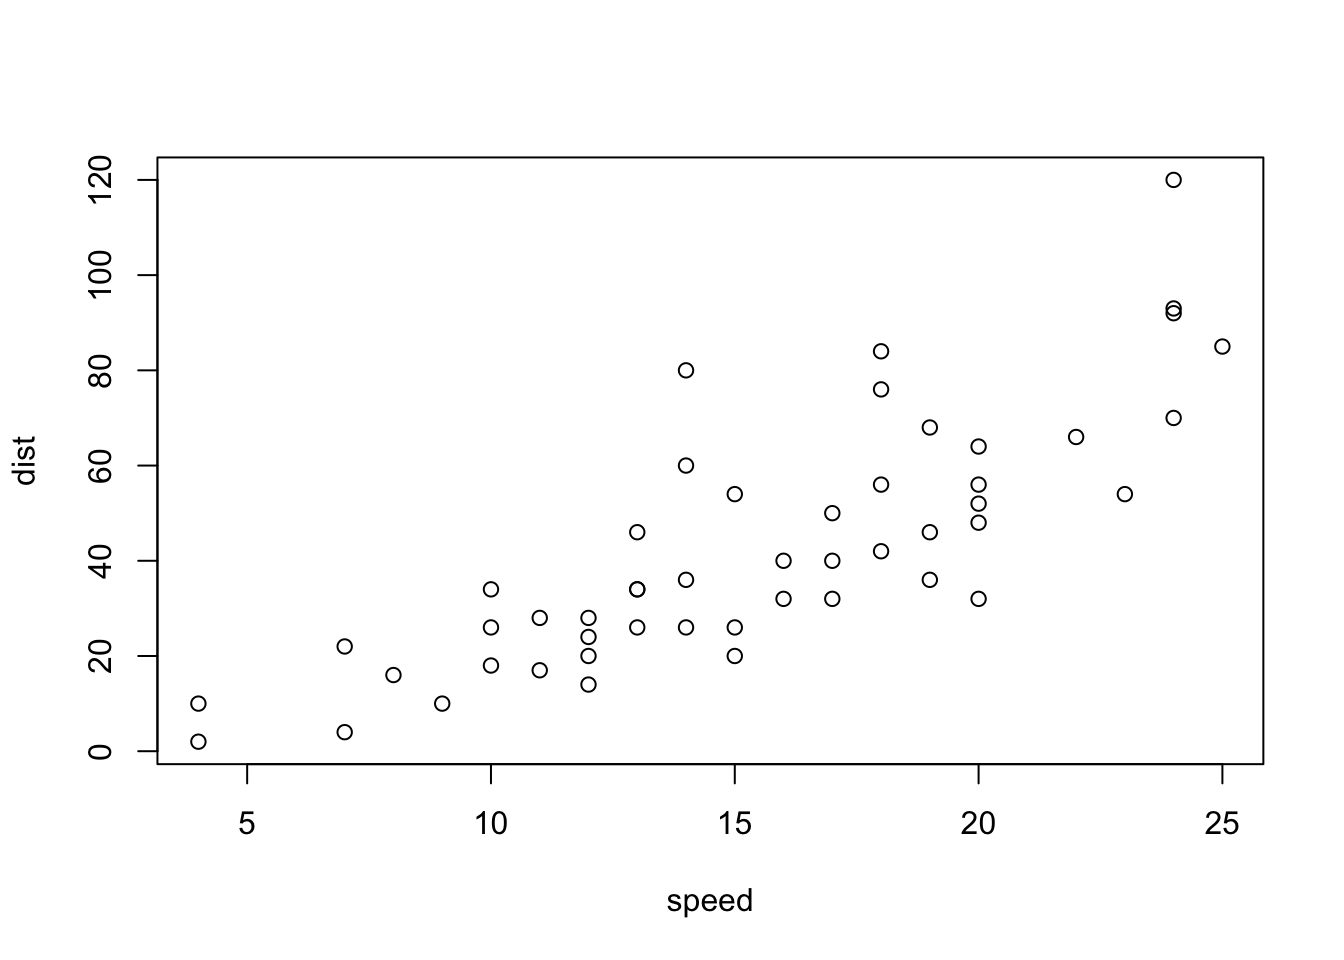
\includegraphics{01_ml_fund_files/figure-latex/unnamed-chunk-2-1.pdf}

\begin{Shaded}
\begin{Highlighting}[]
\CommentTok{#################Business Case##############################}
\NormalTok{employee_attrition_tbl <-}\StringTok{ }\KeywordTok{read_csv}\NormalTok{(}\StringTok{"datasets-1067-1925-WA_Fn-UseC_-HR-Employee-Attrition.csv"}\NormalTok{)}
\end{Highlighting}
\end{Shaded}

\begin{verbatim}
## 
## -- Column specification --------------------------------------------------------
## cols(
##   .default = col_double(),
##   Attrition = col_character(),
##   BusinessTravel = col_character(),
##   Department = col_character(),
##   EducationField = col_character(),
##   Gender = col_character(),
##   JobRole = col_character(),
##   MaritalStatus = col_character(),
##   Over18 = col_character(),
##   OverTime = col_character()
## )
## i Use `spec()` for the full column specifications.
\end{verbatim}

\begin{Shaded}
\begin{Highlighting}[]
\CommentTok{# Business & Data Understanding: Department and Job Role}

\CommentTok{# Data subset}
\NormalTok{dept_job_role_tbl <-}\StringTok{ }\NormalTok{employee_attrition_tbl }\OperatorTok
\StringTok{  }\KeywordTok{select}\NormalTok{(EmployeeNumber, Department, JobRole, PerformanceRating, Attrition)}

\NormalTok{dept_job_role_tbl }\OperatorTok

\StringTok{  }\KeywordTok{group_by}\NormalTok{(Attrition) }\OperatorTok
\StringTok{  }\KeywordTok{summarize}\NormalTok{(}\DataTypeTok{n =} \KeywordTok{n}\NormalTok{()) }\OperatorTok
\StringTok{  }\KeywordTok{ungroup}\NormalTok{() }\OperatorTok
\StringTok{  }\KeywordTok{mutate}\NormalTok{(}\DataTypeTok{pct =}\NormalTok{ n }\OperatorTok{/}\StringTok{ }\KeywordTok{sum}\NormalTok{(n))}
\end{Highlighting}
\end{Shaded}

\begin{verbatim}
## `summarise()` ungrouping output (override with `.groups` argument)
\end{verbatim}

\begin{verbatim}
## # A tibble: 2 x 3
##   Attrition     n   pct
##   <chr>     <int> <dbl>
## 1 No         1233 0.839
## 2 Yes         237 0.161
\end{verbatim}

\begin{Shaded}
\begin{Highlighting}[]
\NormalTok{dept_job_role_tbl }\OperatorTok

\StringTok{  }\CommentTok{# Block 1}
\StringTok{  }\KeywordTok{group_by}\NormalTok{(Department, Attrition) }\OperatorTok
\StringTok{  }\KeywordTok{summarize}\NormalTok{(}\DataTypeTok{n =} \KeywordTok{n}\NormalTok{()) }\OperatorTok
\StringTok{  }\KeywordTok{ungroup}\NormalTok{() }\OperatorTok

\StringTok{  }\CommentTok{# Block 2: Caution: It's easy to inadvertently miss grouping when creating counts & percents within groups}
\StringTok{  }\KeywordTok{group_by}\NormalTok{(Department) }\OperatorTok
\StringTok{  }\KeywordTok{mutate}\NormalTok{(}\DataTypeTok{pct =}\NormalTok{ n }\OperatorTok{/}\StringTok{ }\KeywordTok{sum}\NormalTok{(n))}
\end{Highlighting}
\end{Shaded}

\begin{verbatim}
## `summarise()` regrouping output by 'Department' (override with `.groups` argument)
\end{verbatim}

\begin{verbatim}
## # A tibble: 6 x 4
## # Groups:   Department [3]
##   Department             Attrition     n   pct
##   <chr>                  <chr>     <int> <dbl>
## 1 Human Resources        No           51 0.810
## 2 Human Resources        Yes          12 0.190
## 3 Research & Development No          828 0.862
## 4 Research & Development Yes         133 0.138
## 5 Sales                  No          354 0.794
## 6 Sales                  Yes          92 0.206
\end{verbatim}

\begin{Shaded}
\begin{Highlighting}[]
\NormalTok{dept_job_role_tbl }\OperatorTok

\StringTok{  }\CommentTok{# Block 1}
\StringTok{  }\KeywordTok{group_by}\NormalTok{(Department, JobRole, Attrition) }\OperatorTok
\StringTok{  }\KeywordTok{summarize}\NormalTok{(}\DataTypeTok{n =} \KeywordTok{n}\NormalTok{()) }\OperatorTok
\StringTok{  }\KeywordTok{ungroup}\NormalTok{() }\OperatorTok

\StringTok{  }\CommentTok{# Block 2}
\StringTok{  }\KeywordTok{group_by}\NormalTok{(Department, JobRole) }\OperatorTok
\StringTok{  }\KeywordTok{mutate}\NormalTok{(}\DataTypeTok{pct =}\NormalTok{ n }\OperatorTok{/}\StringTok{ }\KeywordTok{sum}\NormalTok{(n)) }\OperatorTok
\StringTok{  }\KeywordTok{ungroup}\NormalTok{() }\OperatorTok

\StringTok{  }\CommentTok{# Block 3}
\StringTok{  }\KeywordTok{filter}\NormalTok{(Attrition }\OperatorTok\StringTok{ "Yes"}\NormalTok{)}
\end{Highlighting}
\end{Shaded}

\begin{verbatim}
## `summarise()` regrouping output by 'Department', 'JobRole' (override with `.groups` argument)
\end{verbatim}

\begin{verbatim}
## # A tibble: 10 x 5
##    Department             JobRole                   Attrition     n    pct
##    <chr>                  <chr>                     <chr>     <int>  <dbl>
##  1 Human Resources        Human Resources           Yes          12 0.231 
##  2 Research & Development Healthcare Representative Yes           9 0.0687
##  3 Research & Development Laboratory Technician     Yes          62 0.239 
##  4 Research & Development Manager                   Yes           3 0.0556
##  5 Research & Development Manufacturing Director    Yes          10 0.0690
##  6 Research & Development Research Director         Yes           2 0.025 
##  7 Research & Development Research Scientist        Yes          47 0.161 
##  8 Sales                  Manager                   Yes           2 0.0541
##  9 Sales                  Sales Executive           Yes          57 0.175 
## 10 Sales                  Sales Representative      Yes          33 0.398
\end{verbatim}

\begin{Shaded}
\begin{Highlighting}[]
\CommentTok{# Develop KPI}

\NormalTok{dept_job_role_tbl }\OperatorTok

\StringTok{  }\CommentTok{# Block 1}
\StringTok{  }\KeywordTok{group_by}\NormalTok{(Department, JobRole, Attrition) }\OperatorTok
\StringTok{  }\KeywordTok{summarize}\NormalTok{(}\DataTypeTok{n =} \KeywordTok{n}\NormalTok{()) }\OperatorTok
\StringTok{  }\KeywordTok{ungroup}\NormalTok{() }\OperatorTok

\StringTok{  }\CommentTok{# Block 2}
\StringTok{  }\KeywordTok{group_by}\NormalTok{(Department, JobRole) }\OperatorTok
\StringTok{  }\KeywordTok{mutate}\NormalTok{(}\DataTypeTok{pct =}\NormalTok{ n }\OperatorTok{/}\StringTok{ }\KeywordTok{sum}\NormalTok{(n)) }\OperatorTok
\StringTok{  }\KeywordTok{ungroup}\NormalTok{() }\OperatorTok

\StringTok{  }\CommentTok{# Block 3}
\StringTok{  }\KeywordTok{filter}\NormalTok{(Attrition }\OperatorTok\StringTok{ "Yes"}\NormalTok{) }\OperatorTok
\StringTok{  }\KeywordTok{arrange}\NormalTok{(}\KeywordTok{desc}\NormalTok{(pct)) }\OperatorTok
\StringTok{  }\KeywordTok{mutate}\NormalTok{(}
    \DataTypeTok{above_industry_avg =} \KeywordTok{case_when}\NormalTok{(}
\NormalTok{      pct }\OperatorTok{>}\StringTok{ }\FloatTok{0.088} \OperatorTok{~}\StringTok{ "Yes"}\NormalTok{,}
      \OtherTok{TRUE} \OperatorTok{~}\StringTok{ "No"}
\NormalTok{    )}
\NormalTok{  )}
\end{Highlighting}
\end{Shaded}

\begin{verbatim}
## `summarise()` regrouping output by 'Department', 'JobRole' (override with `.groups` argument)
\end{verbatim}

\begin{verbatim}
## # A tibble: 10 x 6
##    Department         JobRole           Attrition     n    pct above_industry_a~
##    <chr>              <chr>             <chr>     <int>  <dbl> <chr>            
##  1 Sales              Sales Representa~ Yes          33 0.398  Yes              
##  2 Research & Develo~ Laboratory Techn~ Yes          62 0.239  Yes              
##  3 Human Resources    Human Resources   Yes          12 0.231  Yes              
##  4 Sales              Sales Executive   Yes          57 0.175  Yes              
##  5 Research & Develo~ Research Scienti~ Yes          47 0.161  Yes              
##  6 Research & Develo~ Manufacturing Di~ Yes          10 0.0690 No               
##  7 Research & Develo~ Healthcare Repre~ Yes           9 0.0687 No               
##  8 Research & Develo~ Manager           Yes           3 0.0556 No               
##  9 Sales              Manager           Yes           2 0.0541 No               
## 10 Research & Develo~ Research Director Yes           2 0.025  No
\end{verbatim}

\begin{Shaded}
\begin{Highlighting}[]
\CommentTok{# Function to calculate attrition cost}
\NormalTok{calculate_attrition_cost <-}\StringTok{ }\ControlFlowTok{function}\NormalTok{(}

  \CommentTok{# Employee}
  \DataTypeTok{n                    =} \DecValTok{1}\NormalTok{,}
  \DataTypeTok{salary               =} \DecValTok{80000}\NormalTok{,}

  \CommentTok{# Direct Costs}
  \DataTypeTok{separation_cost      =} \DecValTok{500}\NormalTok{,}
  \DataTypeTok{vacancy_cost         =} \DecValTok{10000}\NormalTok{,}
  \DataTypeTok{acquisition_cost     =} \DecValTok{4900}\NormalTok{,}
  \DataTypeTok{placement_cost       =} \DecValTok{3500}\NormalTok{,}

  \CommentTok{# Productivity Costs}
  \DataTypeTok{net_revenue_per_employee =} \DecValTok{250000}\NormalTok{,}
  \DataTypeTok{workdays_per_year        =} \DecValTok{240}\NormalTok{,}
  \DataTypeTok{workdays_position_open   =} \DecValTok{40}\NormalTok{,}
  \DataTypeTok{workdays_onboarding      =} \DecValTok{60}\NormalTok{,}
  \DataTypeTok{onboarding_efficiency    =} \FloatTok{0.50}

\NormalTok{) \{}

  \CommentTok{# Direct Costs}
\NormalTok{  direct_cost <-}\StringTok{ }\KeywordTok{sum}\NormalTok{(separation_cost, vacancy_cost, acquisition_cost, placement_cost)}

  \CommentTok{# Lost Productivity Costs}
\NormalTok{  productivity_cost <-}\StringTok{ }\NormalTok{net_revenue_per_employee }\OperatorTok{/}\StringTok{ }\NormalTok{workdays_per_year }\OperatorTok{*}
\StringTok{    }\NormalTok{(workdays_position_open }\OperatorTok{+}\StringTok{ }\NormalTok{workdays_onboarding }\OperatorTok{*}\StringTok{ }\NormalTok{onboarding_efficiency)}

  \CommentTok{# Savings of Salary & Benefits (Cost Reduction)}
\NormalTok{  salary_benefit_reduction <-}\StringTok{ }\NormalTok{salary }\OperatorTok{/}\StringTok{ }\NormalTok{workdays_per_year }\OperatorTok{*}\StringTok{ }\NormalTok{workdays_position_open}

  \CommentTok{# Estimated Turnover Per Employee}
\NormalTok{  cost_per_employee <-}\StringTok{ }\NormalTok{direct_cost }\OperatorTok{+}\StringTok{ }\NormalTok{productivity_cost }\OperatorTok{-}\StringTok{ }\NormalTok{salary_benefit_reduction}

  \CommentTok{# Total Cost of Employee Turnover}
\NormalTok{  total_cost <-}\StringTok{ }\NormalTok{n }\OperatorTok{*}\StringTok{ }\NormalTok{cost_per_employee}

  \KeywordTok{return}\NormalTok{(total_cost)}

\NormalTok{\}}

\KeywordTok{calculate_attrition_cost}\NormalTok{()}
\end{Highlighting}
\end{Shaded}

\begin{verbatim}
## [1] 78483.33
\end{verbatim}

\begin{Shaded}
\begin{Highlighting}[]
\CommentTok{## [1] 78483.33}
\KeywordTok{calculate_attrition_cost}\NormalTok{(}\DecValTok{200}\NormalTok{)}
\end{Highlighting}
\end{Shaded}

\begin{verbatim}
## [1] 15696667
\end{verbatim}

\begin{Shaded}
\begin{Highlighting}[]
\CommentTok{## [1] 15696667}


\NormalTok{dept_job_role_tbl }\OperatorTok

\StringTok{  }\CommentTok{# Block 1}
\StringTok{  }\KeywordTok{group_by}\NormalTok{(Department, JobRole, Attrition) }\OperatorTok
\StringTok{  }\KeywordTok{summarize}\NormalTok{(}\DataTypeTok{n =} \KeywordTok{n}\NormalTok{()) }\OperatorTok
\StringTok{  }\KeywordTok{ungroup}\NormalTok{() }\OperatorTok

\StringTok{  }\CommentTok{# Block 2}
\StringTok{  }\KeywordTok{group_by}\NormalTok{(Department, JobRole) }\OperatorTok
\StringTok{  }\KeywordTok{mutate}\NormalTok{(}\DataTypeTok{pct =}\NormalTok{ n }\OperatorTok{/}\StringTok{ }\KeywordTok{sum}\NormalTok{(n)) }\OperatorTok
\StringTok{  }\KeywordTok{ungroup}\NormalTok{() }\OperatorTok

\StringTok{  }\CommentTok{# Block 3}
\StringTok{  }\KeywordTok{filter}\NormalTok{(Attrition }\OperatorTok\StringTok{ "Yes"}\NormalTok{) }\OperatorTok
\StringTok{  }\KeywordTok{arrange}\NormalTok{(}\KeywordTok{desc}\NormalTok{(pct)) }\OperatorTok
\StringTok{  }\KeywordTok{mutate}\NormalTok{(}
    \DataTypeTok{above_industry_avg =} \KeywordTok{case_when}\NormalTok{(}
\NormalTok{      pct }\OperatorTok{>}\StringTok{ }\FloatTok{0.088} \OperatorTok{~}\StringTok{ "Yes"}\NormalTok{,}
      \OtherTok{TRUE} \OperatorTok{~}\StringTok{ "No"}
\NormalTok{    )}
\NormalTok{  ) }\OperatorTok

\StringTok{  }\CommentTok{# Block 4. Set salaray to 80000 for now}
\StringTok{  }\KeywordTok{mutate}\NormalTok{(}
    \DataTypeTok{cost_of_attrition =} \KeywordTok{calculate_attrition_cost}\NormalTok{(}\DataTypeTok{n =}\NormalTok{ n, }\DataTypeTok{salary =} \DecValTok{80000}\NormalTok{)}
\NormalTok{  )}
\end{Highlighting}
\end{Shaded}

\begin{verbatim}
## `summarise()` regrouping output by 'Department', 'JobRole' (override with `.groups` argument)
\end{verbatim}

\begin{verbatim}
## # A tibble: 10 x 7
##    Department  JobRole  Attrition     n    pct above_industry_~ cost_of_attriti~
##    <chr>       <chr>    <chr>     <int>  <dbl> <chr>                       <dbl>
##  1 Sales       Sales R~ Yes          33 0.398  Yes                      2589950.
##  2 Research &~ Laborat~ Yes          62 0.239  Yes                      4865967.
##  3 Human Reso~ Human R~ Yes          12 0.231  Yes                       941800.
##  4 Sales       Sales E~ Yes          57 0.175  Yes                      4473550.
##  5 Research &~ Researc~ Yes          47 0.161  Yes                      3688717.
##  6 Research &~ Manufac~ Yes          10 0.0690 No                        784833.
##  7 Research &~ Healthc~ Yes           9 0.0687 No                        706350.
##  8 Research &~ Manager  Yes           3 0.0556 No                        235450.
##  9 Sales       Manager  Yes           2 0.0541 No                        156967.
## 10 Research &~ Researc~ Yes           2 0.025  No                        156967.
\end{verbatim}

\begin{Shaded}
\begin{Highlighting}[]
\CommentTok{#Instead of using group and mutate then we should use count for more optimized outputs}
\CommentTok{# Use this}
\NormalTok{dept_job_role_tbl }\OperatorTok

\StringTok{  }\KeywordTok{count}\NormalTok{(Department, JobRole, Attrition)}
\end{Highlighting}
\end{Shaded}

\begin{verbatim}
## # A tibble: 21 x 4
##    Department             JobRole                   Attrition     n
##    <chr>                  <chr>                     <chr>     <int>
##  1 Human Resources        Human Resources           No           40
##  2 Human Resources        Human Resources           Yes          12
##  3 Human Resources        Manager                   No           11
##  4 Research & Development Healthcare Representative No          122
##  5 Research & Development Healthcare Representative Yes           9
##  6 Research & Development Laboratory Technician     No          197
##  7 Research & Development Laboratory Technician     Yes          62
##  8 Research & Development Manager                   No           51
##  9 Research & Development Manager                   Yes           3
## 10 Research & Development Manufacturing Director    No          135
## # ... with 11 more rows
\end{verbatim}

\begin{Shaded}
\begin{Highlighting}[]
\CommentTok{# Use this}
\CommentTok{# Function to convert counts to percentages.}
\NormalTok{count_to_pct <-}\StringTok{ }\ControlFlowTok{function}\NormalTok{(data, ..., }\DataTypeTok{col =}\NormalTok{ n) \{}

  \CommentTok{# capture the dots}
\NormalTok{  grouping_vars_expr <-}\StringTok{ }\KeywordTok{quos}\NormalTok{(...)}
\NormalTok{  col_expr <-}\StringTok{ }\KeywordTok{enquo}\NormalTok{(col)}

\NormalTok{  ret <-}\StringTok{ }\NormalTok{data }\OperatorTok
\StringTok{    }\KeywordTok{group_by}\NormalTok{(}\OperatorTok{!!!}\StringTok{ }\NormalTok{grouping_vars_expr) }\OperatorTok
\StringTok{    }\KeywordTok{mutate}\NormalTok{(}\DataTypeTok{pct =}\NormalTok{ (}\OperatorTok{!!}\StringTok{ }\NormalTok{col_expr) }\OperatorTok{/}\StringTok{ }\KeywordTok{sum}\NormalTok{(}\OperatorTok{!!}\StringTok{ }\NormalTok{col_expr)) }\OperatorTok
\StringTok{    }\KeywordTok{ungroup}\NormalTok{()}

  \KeywordTok{return}\NormalTok{(ret)}

\NormalTok{\}}

\CommentTok{# This is way shorter and more flexible}
\NormalTok{dept_job_role_tbl }\OperatorTok
\StringTok{  }\KeywordTok{count}\NormalTok{(JobRole, Attrition) }\OperatorTok
\StringTok{  }\KeywordTok{count_to_pct}\NormalTok{(JobRole)}
\end{Highlighting}
\end{Shaded}

\begin{verbatim}
## # A tibble: 18 x 4
##    JobRole                   Attrition     n    pct
##    <chr>                     <chr>     <int>  <dbl>
##  1 Healthcare Representative No          122 0.931 
##  2 Healthcare Representative Yes           9 0.0687
##  3 Human Resources           No           40 0.769 
##  4 Human Resources           Yes          12 0.231 
##  5 Laboratory Technician     No          197 0.761 
##  6 Laboratory Technician     Yes          62 0.239 
##  7 Manager                   No           97 0.951 
##  8 Manager                   Yes           5 0.0490
##  9 Manufacturing Director    No          135 0.931 
## 10 Manufacturing Director    Yes          10 0.0690
## 11 Research Director         No           78 0.975 
## 12 Research Director         Yes           2 0.025 
## 13 Research Scientist        No          245 0.839 
## 14 Research Scientist        Yes          47 0.161 
## 15 Sales Executive           No          269 0.825 
## 16 Sales Executive           Yes          57 0.175 
## 17 Sales Representative      No           50 0.602 
## 18 Sales Representative      Yes          33 0.398
\end{verbatim}

\begin{Shaded}
\begin{Highlighting}[]
\NormalTok{dept_job_role_tbl }\OperatorTok
\StringTok{  }\KeywordTok{count}\NormalTok{(Department, JobRole, Attrition) }\OperatorTok
\StringTok{  }\KeywordTok{count_to_pct}\NormalTok{(Department, JobRole)}
\end{Highlighting}
\end{Shaded}

\begin{verbatim}
## # A tibble: 21 x 5
##    Department             JobRole                   Attrition     n    pct
##    <chr>                  <chr>                     <chr>     <int>  <dbl>
##  1 Human Resources        Human Resources           No           40 0.769 
##  2 Human Resources        Human Resources           Yes          12 0.231 
##  3 Human Resources        Manager                   No           11 1     
##  4 Research & Development Healthcare Representative No          122 0.931 
##  5 Research & Development Healthcare Representative Yes           9 0.0687
##  6 Research & Development Laboratory Technician     No          197 0.761 
##  7 Research & Development Laboratory Technician     Yes          62 0.239 
##  8 Research & Development Manager                   No           51 0.944 
##  9 Research & Development Manager                   Yes           3 0.0556
## 10 Research & Development Manufacturing Director    No          135 0.931 
## # ... with 11 more rows
\end{verbatim}

\begin{Shaded}
\begin{Highlighting}[]
\NormalTok{assess_attrition <-}\StringTok{ }\ControlFlowTok{function}\NormalTok{(data, attrition_col, attrition_value, baseline_pct) \{}

\NormalTok{  attrition_col_expr <-}\StringTok{ }\KeywordTok{enquo}\NormalTok{(attrition_col)}

\NormalTok{  data }\OperatorTok

\StringTok{    }\CommentTok{# Use parenthesis () to give tidy eval evaluation priority}
\StringTok{    }\KeywordTok{filter}\NormalTok{((}\OperatorTok{!!}\StringTok{ }\NormalTok{attrition_col_expr) }\OperatorTok\StringTok{ }\NormalTok{attrition_value) }\OperatorTok
\StringTok{    }\KeywordTok{arrange}\NormalTok{(}\KeywordTok{desc}\NormalTok{(pct)) }\OperatorTok
\StringTok{    }\KeywordTok{mutate}\NormalTok{(}
      \CommentTok{# Function inputs in numeric format (e.g. baseline_pct = 0.088 don't require tidy eval)}
      \DataTypeTok{above_industry_avg =} \KeywordTok{case_when}\NormalTok{(}
\NormalTok{        pct }\OperatorTok{>}\StringTok{ }\NormalTok{baseline_pct }\OperatorTok{~}\StringTok{ "Yes"}\NormalTok{,}
        \OtherTok{TRUE} \OperatorTok{~}\StringTok{ "No"}
\NormalTok{      )}
\NormalTok{    )}

\NormalTok{\}}


\NormalTok{dept_job_role_tbl }\OperatorTok

\StringTok{  }\KeywordTok{count}\NormalTok{(Department, JobRole, Attrition) }\OperatorTok
\StringTok{  }\KeywordTok{count_to_pct}\NormalTok{(Department, JobRole) }\OperatorTok
\StringTok{  }\KeywordTok{assess_attrition}\NormalTok{(Attrition, }\DataTypeTok{attrition_value =} \StringTok{"Yes"}\NormalTok{, }\DataTypeTok{baseline_pct =} \FloatTok{0.088}\NormalTok{) }\OperatorTok
\StringTok{  }\KeywordTok{mutate}\NormalTok{(}
    \DataTypeTok{cost_of_attrition =} \KeywordTok{calculate_attrition_cost}\NormalTok{(}\DataTypeTok{n =}\NormalTok{ n, }\DataTypeTok{salary =} \DecValTok{80000}\NormalTok{)}
\NormalTok{  )}
\end{Highlighting}
\end{Shaded}

\begin{verbatim}
## # A tibble: 10 x 7
##    Department  JobRole  Attrition     n    pct above_industry_~ cost_of_attriti~
##    <chr>       <chr>    <chr>     <int>  <dbl> <chr>                       <dbl>
##  1 Sales       Sales R~ Yes          33 0.398  Yes                      2589950.
##  2 Research &~ Laborat~ Yes          62 0.239  Yes                      4865967.
##  3 Human Reso~ Human R~ Yes          12 0.231  Yes                       941800.
##  4 Sales       Sales E~ Yes          57 0.175  Yes                      4473550.
##  5 Research &~ Researc~ Yes          47 0.161  Yes                      3688717.
##  6 Research &~ Manufac~ Yes          10 0.0690 No                        784833.
##  7 Research &~ Healthc~ Yes           9 0.0687 No                        706350.
##  8 Research &~ Manager  Yes           3 0.0556 No                        235450.
##  9 Sales       Manager  Yes           2 0.0541 No                        156967.
## 10 Research &~ Researc~ Yes           2 0.025  No                        156967.
\end{verbatim}

\begin{Shaded}
\begin{Highlighting}[]
\NormalTok{dept_job_role_tbl }\OperatorTok

\StringTok{  }\KeywordTok{count}\NormalTok{(Department, JobRole, Attrition) }\OperatorTok
\StringTok{  }\KeywordTok{count_to_pct}\NormalTok{(Department, JobRole) }\OperatorTok
\StringTok{  }\KeywordTok{assess_attrition}\NormalTok{(Attrition, }\DataTypeTok{attrition_value =} \StringTok{"Yes"}\NormalTok{, }\DataTypeTok{baseline_pct =} \FloatTok{0.088}\NormalTok{) }\OperatorTok
\StringTok{  }\KeywordTok{mutate}\NormalTok{(}
    \DataTypeTok{cost_of_attrition =} \KeywordTok{calculate_attrition_cost}\NormalTok{(}\DataTypeTok{n =}\NormalTok{ n, }\DataTypeTok{salary =} \DecValTok{80000}\NormalTok{)}
\NormalTok{  ) }\OperatorTok

\StringTok{  }\CommentTok{# Data Manipulation}
\StringTok{  }\KeywordTok{mutate}\NormalTok{(}\DataTypeTok{name =} \KeywordTok{str_c}\NormalTok{(Department, JobRole, }\DataTypeTok{sep =} \StringTok{": "}\NormalTok{) }\OperatorTok\StringTok{ }\KeywordTok{as_factor}\NormalTok{()) }\OperatorTok

\StringTok{  }\CommentTok{# Check levels}
\StringTok{  }\CommentTok{# pull(name) %>%}
\StringTok{  }\CommentTok{# levels()}

\StringTok{  }\KeywordTok{mutate}\NormalTok{(}\DataTypeTok{name      =} \KeywordTok{fct_reorder}\NormalTok{(name, cost_of_attrition)) }\OperatorTok
\StringTok{  }\KeywordTok{mutate}\NormalTok{(}\DataTypeTok{cost_text =} \KeywordTok{str_c}\NormalTok{(}\StringTok{"$"}\NormalTok{, }\KeywordTok{format}\NormalTok{(cost_of_attrition }\OperatorTok{/}\StringTok{ }\FloatTok{1e6}\NormalTok{, }\DataTypeTok{digits =} \DecValTok{2}\NormalTok{),}
                           \StringTok{"M"}\NormalTok{, }\DataTypeTok{sep =} \StringTok{""}\NormalTok{)) }\OperatorTok

\StringTok{  }\CommentTok{#Plotting}
\StringTok{  }\KeywordTok{ggplot}\NormalTok{(}\KeywordTok{aes}\NormalTok{(cost_of_attrition, }\DataTypeTok{y =}\NormalTok{ name)) }\OperatorTok{+}
\StringTok{  }\KeywordTok{geom_segment}\NormalTok{(}\KeywordTok{aes}\NormalTok{(}\DataTypeTok{xend =} \DecValTok{0}\NormalTok{, }\DataTypeTok{yend =}\NormalTok{ name),    }\DataTypeTok{color =} \StringTok{"#2dc6d6"}\NormalTok{) }\OperatorTok{+}
\StringTok{  }\KeywordTok{geom_point}\NormalTok{(  }\KeywordTok{aes}\NormalTok{(}\DataTypeTok{size =}\NormalTok{ cost_of_attrition), }\DataTypeTok{color =} \StringTok{"#2dc6d6"}\NormalTok{) }\OperatorTok{+}
\StringTok{  }\KeywordTok{scale_x_continuous}\NormalTok{(}\DataTypeTok{labels =}\NormalTok{ scales}\OperatorTok{::}\NormalTok{dollar) }\OperatorTok{+}
\StringTok{  }\KeywordTok{geom_label}\NormalTok{(}\KeywordTok{aes}\NormalTok{(}\DataTypeTok{label =}\NormalTok{ cost_text, }\DataTypeTok{size =}\NormalTok{ cost_of_attrition),}
             \DataTypeTok{hjust =} \StringTok{"inward"}\NormalTok{, }\DataTypeTok{color =} \StringTok{"#2dc6d6"}\NormalTok{) }\OperatorTok{+}
\StringTok{  }\KeywordTok{scale_size}\NormalTok{(}\DataTypeTok{range =} \KeywordTok{c}\NormalTok{(}\DecValTok{3}\NormalTok{, }\DecValTok{5}\NormalTok{)) }\OperatorTok{+}
\StringTok{  }\KeywordTok{labs}\NormalTok{(}\DataTypeTok{title =} \StringTok{"Estimated cost of Attrition: By Dept and Job Role"}\NormalTok{,}
       \DataTypeTok{y =} \StringTok{""}\NormalTok{,}
       \DataTypeTok{x =} \StringTok{"Cost of attrition"}\NormalTok{) }\OperatorTok{+}
\StringTok{  }\KeywordTok{theme}\NormalTok{(}\DataTypeTok{legend.position =} \StringTok{"none"}\NormalTok{)}
\end{Highlighting}
\end{Shaded}

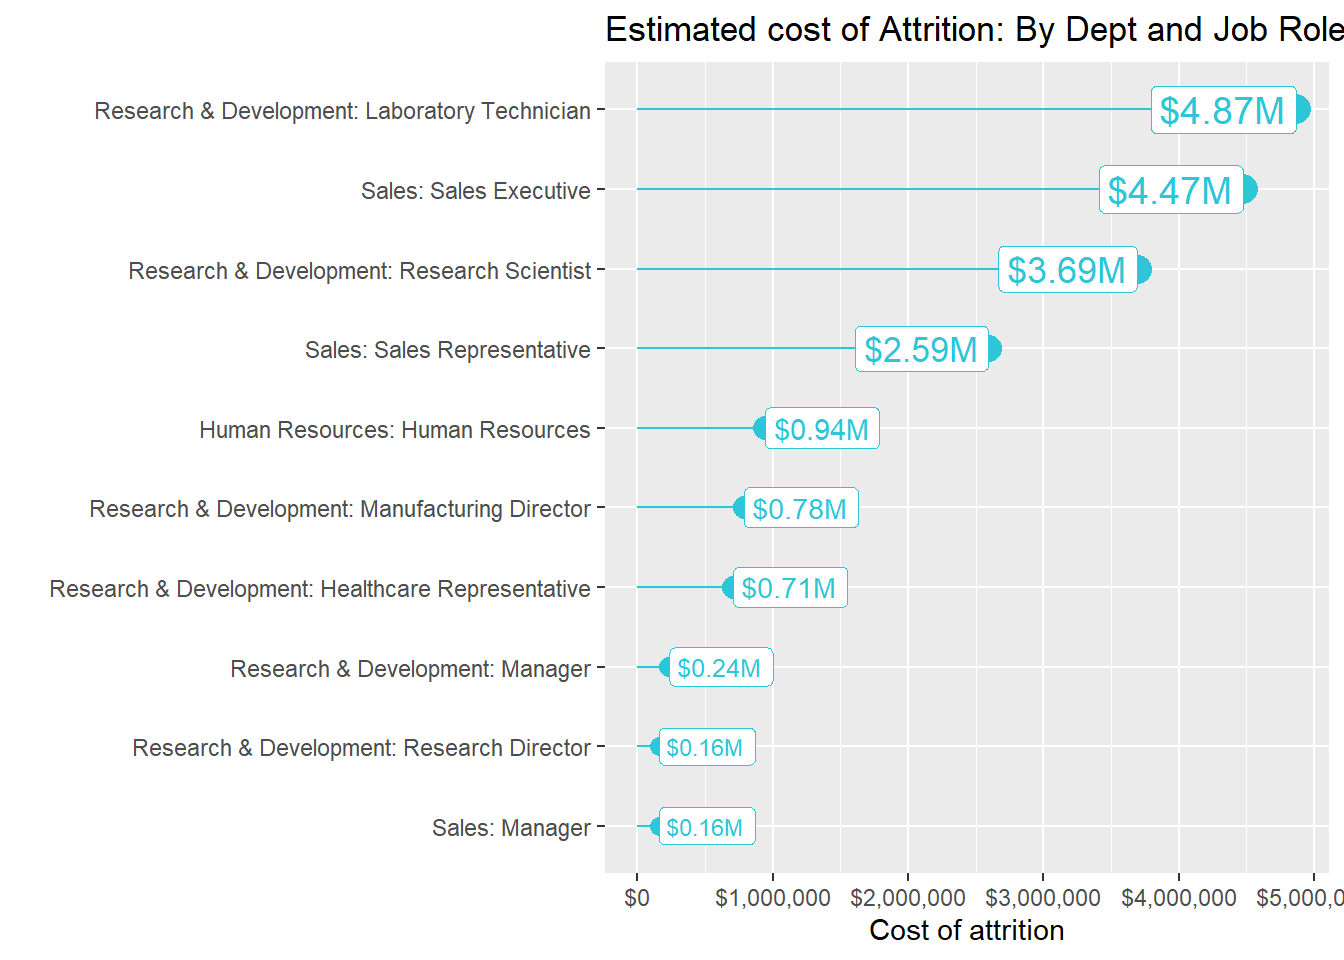
\includegraphics{01_ml_fund_files/figure-latex/unnamed-chunk-2-2.pdf}

\begin{Shaded}
\begin{Highlighting}[]
\CommentTok{# This will return a quoted result}
\KeywordTok{colnames}\NormalTok{(dept_job_role_tbl)[[}\DecValTok{1}\NormalTok{]]}
\end{Highlighting}
\end{Shaded}

\begin{verbatim}
## [1] "EmployeeNumber"
\end{verbatim}

\begin{Shaded}
\begin{Highlighting}[]
\CommentTok{## "EmployeeNumber"}

\CommentTok{# This will become an unquoted expression}
\NormalTok{rlang}\OperatorTok{::}\KeywordTok{sym}\NormalTok{(}\KeywordTok{colnames}\NormalTok{(dept_job_role_tbl)[[}\DecValTok{1}\NormalTok{]])}
\end{Highlighting}
\end{Shaded}

\begin{verbatim}
## EmployeeNumber
\end{verbatim}

\begin{Shaded}
\begin{Highlighting}[]
\CommentTok{## EmployeeNumber}

\CommentTok{# quos() captures it and turns it into a quosure, which is a list}
\CommentTok{# Will be evaluated at the time we use the double !! later on in the code.}
\CommentTok{# Then it will turn it into EmployeeNumber}
\KeywordTok{quos}\NormalTok{(rlang}\OperatorTok{::}\KeywordTok{sym}\NormalTok{(}\KeywordTok{colnames}\NormalTok{(employee_attrition_tbl)[[}\DecValTok{1}\NormalTok{]]))}
\end{Highlighting}
\end{Shaded}

\begin{verbatim}
## <list_of<quosure>>
## 
## [[1]]
## <quosure>
## expr: ^rlang::sym(colnames(employee_attrition_tbl)[[1]])
## env:  global
\end{verbatim}

\begin{Shaded}
\begin{Highlighting}[]
\CommentTok{## <list_of<quosure>>}
\CommentTok{##}
\CommentTok{## [[1]]}
\CommentTok{## <quosure>}
\CommentTok{## expr: ^rlang::sym(colnames(employee_attrition_tbl)[[1]])}
\CommentTok{## env:  global}

\CommentTok{# If the user supplies two different columns such as Department and Job Role}
\CommentTok{# or if the user does not supply a column the length will be different}
\KeywordTok{quos}\NormalTok{(Department, JobRole)}
\end{Highlighting}
\end{Shaded}

\begin{verbatim}
## <list_of<quosure>>
## 
## [[1]]
## <quosure>
## expr: ^Department
## env:  global
## 
## [[2]]
## <quosure>
## expr: ^JobRole
## env:  global
\end{verbatim}

\begin{Shaded}
\begin{Highlighting}[]
\KeywordTok{quos}\NormalTok{(Department, JobRole) }\OperatorTok\StringTok{ }\KeywordTok{length}\NormalTok{()}
\end{Highlighting}
\end{Shaded}

\begin{verbatim}
## [1] 2
\end{verbatim}

\begin{Shaded}
\begin{Highlighting}[]
\CommentTok{## 2}
\KeywordTok{quos}\NormalTok{() }\OperatorTok\StringTok{ }\NormalTok{length}
\end{Highlighting}
\end{Shaded}

\begin{verbatim}
## [1] 0
\end{verbatim}

\begin{Shaded}
\begin{Highlighting}[]
\CommentTok{## 0}

\CommentTok{# Function to plot attrition}
\NormalTok{plot_attrition <-}\StringTok{ }\ControlFlowTok{function}\NormalTok{(data,}
\NormalTok{                           ...,}
\NormalTok{                           .value,}
                           \DataTypeTok{fct_reorder =} \OtherTok{TRUE}\NormalTok{,}
                           \DataTypeTok{fct_rev     =} \OtherTok{FALSE}\NormalTok{,}
                           \DataTypeTok{include_lbl =} \OtherTok{TRUE}\NormalTok{,}
                           \DataTypeTok{color       =} \StringTok{"#2dc6d6"}\NormalTok{,}
                           \DataTypeTok{units       =} \KeywordTok{c}\NormalTok{(}\StringTok{"0"}\NormalTok{, }\StringTok{"K"}\NormalTok{, }\StringTok{"M"}\NormalTok{)) \{}

  \CommentTok{### Inputs}
\NormalTok{  group_vars_expr   <-}\StringTok{ }\KeywordTok{quos}\NormalTok{(...)}

  \CommentTok{# If the user does not supply anything,}
  \CommentTok{# this takes the first column of the supplied data}
  \ControlFlowTok{if}\NormalTok{ (}\KeywordTok{length}\NormalTok{(group_vars_expr) }\OperatorTok{==}\StringTok{ }\DecValTok{0}\NormalTok{) \{}
\NormalTok{    group_vars_expr <-}\StringTok{ }\KeywordTok{quos}\NormalTok{(rlang}\OperatorTok{::}\KeywordTok{sym}\NormalTok{(}\KeywordTok{colnames}\NormalTok{(data)[[}\DecValTok{1}\NormalTok{]]))}
\NormalTok{  \}}

\NormalTok{  value_expr <-}\StringTok{ }\KeywordTok{enquo}\NormalTok{(.value)}

\NormalTok{  units_val  <-}\StringTok{ }\ControlFlowTok{switch}\NormalTok{(units[[}\DecValTok{1}\NormalTok{]],}
                       \StringTok{"M"}\NormalTok{ =}\StringTok{ }\FloatTok{1e6}\NormalTok{,}
                       \StringTok{"K"}\NormalTok{ =}\StringTok{ }\FloatTok{1e3}\NormalTok{,}
                       \StringTok{"0"}\NormalTok{ =}\StringTok{ }\DecValTok{1}\NormalTok{)}
  \ControlFlowTok{if}\NormalTok{ (units[[}\DecValTok{1}\NormalTok{]] }\OperatorTok{==}\StringTok{ "0"}\NormalTok{) units <-}\StringTok{ ""}

  \CommentTok{# Data Manipulation}
  \CommentTok{# This is a so called Function Factory (a function that produces a function)}
\NormalTok{  usd <-}\StringTok{ }\NormalTok{scales}\OperatorTok{::}\KeywordTok{dollar_format}\NormalTok{(}\DataTypeTok{prefix =} \StringTok{"$"}\NormalTok{, }\DataTypeTok{largest_with_cents =} \FloatTok{1e3}\NormalTok{)}

  \CommentTok{# Create the axis labels and values for the plot}
\NormalTok{  data_manipulated <-}\StringTok{ }\NormalTok{data }\OperatorTok
\StringTok{    }\KeywordTok{mutate}\NormalTok{(}\DataTypeTok{name =} \KeywordTok{str_c}\NormalTok{(}\OperatorTok{!!!}\StringTok{ }\NormalTok{group_vars_expr, }\DataTypeTok{sep =} \StringTok{": "}\NormalTok{) }\OperatorTok\StringTok{ }\KeywordTok{as_factor}\NormalTok{()) }\OperatorTok
\StringTok{    }\KeywordTok{mutate}\NormalTok{(}\DataTypeTok{value_text =} \KeywordTok{str_c}\NormalTok{(}\KeywordTok{usd}\NormalTok{(}\OperatorTok{!!}\StringTok{ }\NormalTok{value_expr }\OperatorTok{/}\StringTok{ }\NormalTok{units_val),}
\NormalTok{                              units[[}\DecValTok{1}\NormalTok{]], }\DataTypeTok{sep =} \StringTok{""}\NormalTok{))}


  \CommentTok{# Order the labels on the y-axis according to the input}
  \ControlFlowTok{if}\NormalTok{ (fct_reorder) \{}
\NormalTok{    data_manipulated <-}\StringTok{ }\NormalTok{data_manipulated }\OperatorTok
\StringTok{      }\KeywordTok{mutate}\NormalTok{(}\DataTypeTok{name =}\NormalTok{ forcats}\OperatorTok{::}\KeywordTok{fct_reorder}\NormalTok{(name, }\OperatorTok{!!}\StringTok{ }\NormalTok{value_expr)) }\OperatorTok
\StringTok{      }\KeywordTok{arrange}\NormalTok{(name)}
\NormalTok{  \}}

  \ControlFlowTok{if}\NormalTok{ (fct_rev) \{}
\NormalTok{    data_manipulated <-}\StringTok{ }\NormalTok{data_manipulated }\OperatorTok
\StringTok{      }\KeywordTok{mutate}\NormalTok{(}\DataTypeTok{name =}\NormalTok{ forcats}\OperatorTok{::}\KeywordTok{fct_rev}\NormalTok{(name)) }\OperatorTok
\StringTok{      }\KeywordTok{arrange}\NormalTok{(name)}
\NormalTok{  \}}

  \CommentTok{# Visualization}
\NormalTok{  g <-}\StringTok{ }\NormalTok{data_manipulated }\OperatorTok

\StringTok{    }\CommentTok{# "name" is a column name generated by our function internally as part of the data manipulation task}
\StringTok{    }\KeywordTok{ggplot}\NormalTok{(}\KeywordTok{aes}\NormalTok{(}\DataTypeTok{x =}\NormalTok{ (}\OperatorTok{!!}\StringTok{ }\NormalTok{value_expr), }\DataTypeTok{y =}\NormalTok{ name)) }\OperatorTok{+}
\StringTok{    }\KeywordTok{geom_segment}\NormalTok{(}\KeywordTok{aes}\NormalTok{(}\DataTypeTok{xend =} \DecValTok{0}\NormalTok{, }\DataTypeTok{yend =}\NormalTok{ name), }\DataTypeTok{color =}\NormalTok{ color) }\OperatorTok{+}
\StringTok{    }\KeywordTok{geom_point}\NormalTok{(}\KeywordTok{aes}\NormalTok{(}\DataTypeTok{size =} \OperatorTok{!!}\StringTok{ }\NormalTok{value_expr), }\DataTypeTok{color =}\NormalTok{ color) }\OperatorTok{+}
\StringTok{    }\KeywordTok{scale_x_continuous}\NormalTok{(}\DataTypeTok{labels =}\NormalTok{ scales}\OperatorTok{::}\NormalTok{dollar) }\OperatorTok{+}
\StringTok{    }\KeywordTok{scale_size}\NormalTok{(}\DataTypeTok{range =} \KeywordTok{c}\NormalTok{(}\DecValTok{3}\NormalTok{, }\DecValTok{5}\NormalTok{)) }\OperatorTok{+}
\StringTok{    }\KeywordTok{theme}\NormalTok{(}\DataTypeTok{legend.position =} \StringTok{"none"}\NormalTok{)}

  \CommentTok{# Plot labels if TRUE}
  \ControlFlowTok{if}\NormalTok{ (include_lbl) \{}
\NormalTok{    g <-}\StringTok{ }\NormalTok{g }\OperatorTok{+}
\StringTok{      }\KeywordTok{geom_label}\NormalTok{(}\KeywordTok{aes}\NormalTok{(}\DataTypeTok{label =}\NormalTok{ value_text, }\DataTypeTok{size =} \OperatorTok{!!}\StringTok{ }\NormalTok{value_expr),}
                 \DataTypeTok{hjust =} \StringTok{"inward"}\NormalTok{, }\DataTypeTok{color =}\NormalTok{ color)}
\NormalTok{  \}}

  \KeywordTok{return}\NormalTok{(g)}

\NormalTok{\}}

\NormalTok{dept_job_role_tbl }\OperatorTok

\StringTok{  }\CommentTok{# Select columns}
\StringTok{  }\KeywordTok{count}\NormalTok{(Department, JobRole, Attrition) }\OperatorTok
\StringTok{  }\KeywordTok{count_to_pct}\NormalTok{(Department, JobRole) }\OperatorTok

\StringTok{  }\KeywordTok{assess_attrition}\NormalTok{(Attrition, }\DataTypeTok{attrition_value =} \StringTok{"Yes"}\NormalTok{, }\DataTypeTok{baseline_pct =} \FloatTok{0.088}\NormalTok{) }\OperatorTok
\StringTok{  }\KeywordTok{mutate}\NormalTok{(}
    \DataTypeTok{cost_of_attrition =} \KeywordTok{calculate_attrition_cost}\NormalTok{(}\DataTypeTok{n =}\NormalTok{ n, }\DataTypeTok{salary =} \DecValTok{80000}\NormalTok{)}
\NormalTok{  ) }\OperatorTok

\StringTok{  }\CommentTok{# Select columns}
\StringTok{  }\KeywordTok{plot_attrition}\NormalTok{(Department, JobRole, }\DataTypeTok{.value =}\NormalTok{ cost_of_attrition,}
                 \DataTypeTok{units =} \StringTok{"M"}\NormalTok{) }\OperatorTok{+}
\StringTok{  }\KeywordTok{labs}\NormalTok{(}
    \DataTypeTok{title =} \StringTok{"Estimated Cost of Attrition by Job Role"}\NormalTok{,}
    \DataTypeTok{x =} \StringTok{"Cost of Attrition"}\NormalTok{,}
    \DataTypeTok{subtitle =} \StringTok{"Looks like Sales Executive and Labaratory Technician are the biggest drivers of cost"}
\NormalTok{  )}
\end{Highlighting}
\end{Shaded}

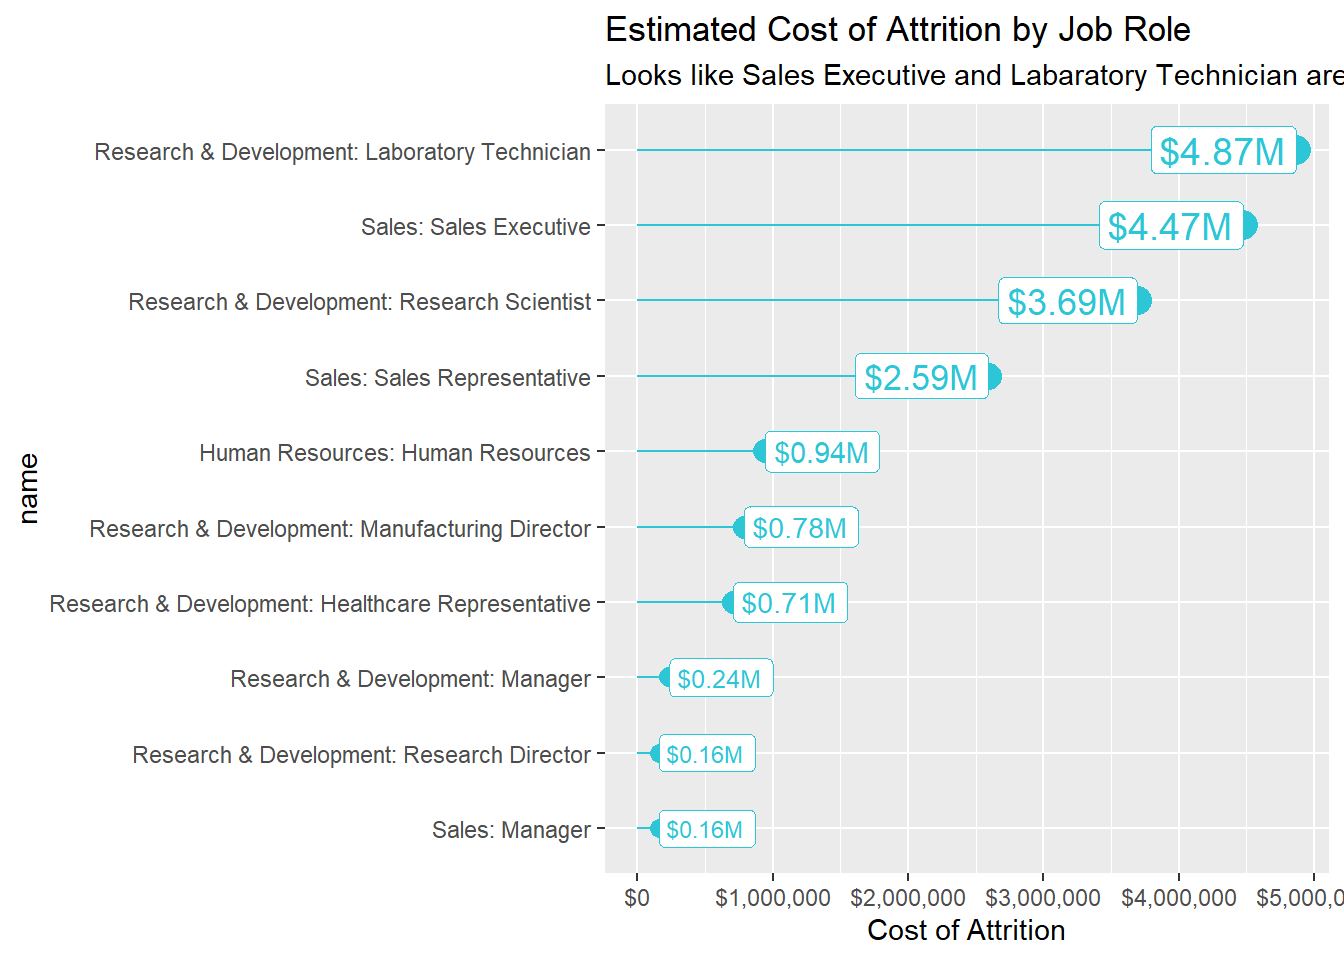
\includegraphics{01_ml_fund_files/figure-latex/unnamed-chunk-2-3.pdf}

\begin{Shaded}
\begin{Highlighting}[]
\NormalTok{path_data_definitions <-}\StringTok{ "data_definitions.xlsx"}
\NormalTok{definitions_raw_tbl   <-}\StringTok{ }\KeywordTok{read_excel}\NormalTok{(path_data_definitions, }\DataTypeTok{sheet =} \DecValTok{1}\NormalTok{, }\DataTypeTok{col_names =} \OtherTok{FALSE}\NormalTok{)}
\end{Highlighting}
\end{Shaded}

\begin{verbatim}
## New names:
## * `` -> ...1
## * `` -> ...2
\end{verbatim}

\begin{Shaded}
\begin{Highlighting}[]
\NormalTok{employee_attrition_tbl}
\end{Highlighting}
\end{Shaded}

\begin{verbatim}
## # A tibble: 1,470 x 35
##      Age Attrition BusinessTravel DailyRate Department DistanceFromHome
##    <dbl> <chr>     <chr>              <dbl> <chr>                 <dbl>
##  1    41 Yes       Travel_Rarely       1102 Sales                     1
##  2    49 No        Travel_Freque~       279 Research ~                8
##  3    37 Yes       Travel_Rarely       1373 Research ~                2
##  4    33 No        Travel_Freque~      1392 Research ~                3
##  5    27 No        Travel_Rarely        591 Research ~                2
##  6    32 No        Travel_Freque~      1005 Research ~                2
##  7    59 No        Travel_Rarely       1324 Research ~                3
##  8    30 No        Travel_Rarely       1358 Research ~               24
##  9    38 No        Travel_Freque~       216 Research ~               23
## 10    36 No        Travel_Rarely       1299 Research ~               27
## # ... with 1,460 more rows, and 29 more variables: Education <dbl>,
## #   EducationField <chr>, EmployeeCount <dbl>, EmployeeNumber <dbl>,
## #   EnvironmentSatisfaction <dbl>, Gender <chr>, HourlyRate <dbl>,
## #   JobInvolvement <dbl>, JobLevel <dbl>, JobRole <chr>, JobSatisfaction <dbl>,
## #   MaritalStatus <chr>, MonthlyIncome <dbl>, MonthlyRate <dbl>,
## #   NumCompaniesWorked <dbl>, Over18 <chr>, OverTime <chr>,
## #   PercentSalaryHike <dbl>, PerformanceRating <dbl>,
## #   RelationshipSatisfaction <dbl>, StandardHours <dbl>,
## #   StockOptionLevel <dbl>, TotalWorkingYears <dbl>,
## #   TrainingTimesLastYear <dbl>, WorkLifeBalance <dbl>, YearsAtCompany <dbl>,
## #   YearsInCurrentRole <dbl>, YearsSinceLastPromotion <dbl>,
## #   YearsWithCurrManager <dbl>
\end{verbatim}

\begin{Shaded}
\begin{Highlighting}[]
\NormalTok{path_data_definitions <-}\StringTok{ "data_definitions.xlsx"}
\NormalTok{definitions_raw_tbl   <-}\StringTok{ }\KeywordTok{read_excel}\NormalTok{(path_data_definitions, }\DataTypeTok{sheet =} \DecValTok{1}\NormalTok{, }\DataTypeTok{col_names =} \OtherTok{FALSE}\NormalTok{)}
\end{Highlighting}
\end{Shaded}

\begin{verbatim}
## New names:
## * `` -> ...1
## * `` -> ...2
\end{verbatim}

\begin{Shaded}
\begin{Highlighting}[]
\NormalTok{employee_attrition_tbl}
\end{Highlighting}
\end{Shaded}

\begin{verbatim}
## # A tibble: 1,470 x 35
##      Age Attrition BusinessTravel DailyRate Department DistanceFromHome
##    <dbl> <chr>     <chr>              <dbl> <chr>                 <dbl>
##  1    41 Yes       Travel_Rarely       1102 Sales                     1
##  2    49 No        Travel_Freque~       279 Research ~                8
##  3    37 Yes       Travel_Rarely       1373 Research ~                2
##  4    33 No        Travel_Freque~      1392 Research ~                3
##  5    27 No        Travel_Rarely        591 Research ~                2
##  6    32 No        Travel_Freque~      1005 Research ~                2
##  7    59 No        Travel_Rarely       1324 Research ~                3
##  8    30 No        Travel_Rarely       1358 Research ~               24
##  9    38 No        Travel_Freque~       216 Research ~               23
## 10    36 No        Travel_Rarely       1299 Research ~               27
## # ... with 1,460 more rows, and 29 more variables: Education <dbl>,
## #   EducationField <chr>, EmployeeCount <dbl>, EmployeeNumber <dbl>,
## #   EnvironmentSatisfaction <dbl>, Gender <chr>, HourlyRate <dbl>,
## #   JobInvolvement <dbl>, JobLevel <dbl>, JobRole <chr>, JobSatisfaction <dbl>,
## #   MaritalStatus <chr>, MonthlyIncome <dbl>, MonthlyRate <dbl>,
## #   NumCompaniesWorked <dbl>, Over18 <chr>, OverTime <chr>,
## #   PercentSalaryHike <dbl>, PerformanceRating <dbl>,
## #   RelationshipSatisfaction <dbl>, StandardHours <dbl>,
## #   StockOptionLevel <dbl>, TotalWorkingYears <dbl>,
## #   TrainingTimesLastYear <dbl>, WorkLifeBalance <dbl>, YearsAtCompany <dbl>,
## #   YearsInCurrentRole <dbl>, YearsSinceLastPromotion <dbl>,
## #   YearsWithCurrManager <dbl>
\end{verbatim}

\begin{Shaded}
\begin{Highlighting}[]
\CommentTok{# Step 1: Data Summarization -----}

\KeywordTok{skim}\NormalTok{(employee_attrition_tbl)}
\end{Highlighting}
\end{Shaded}

\begin{longtable}[]{@{}ll@{}}
\caption{Data summary}\tabularnewline
\toprule
\endhead
Name & employee\_attrition\_tbl\tabularnewline
Number of rows & 1470\tabularnewline
Number of columns & 35\tabularnewline
\_\_\_\_\_\_\_\_\_\_\_\_\_\_\_\_\_\_\_\_\_\_\_ &\tabularnewline
Column type frequency: &\tabularnewline
character & 9\tabularnewline
numeric & 26\tabularnewline
\_\_\_\_\_\_\_\_\_\_\_\_\_\_\_\_\_\_\_\_\_\_\_\_ &\tabularnewline
Group variables & None\tabularnewline
\bottomrule
\end{longtable}

\textbf{Variable type: character}

\begin{longtable}[]{@{}lrrrrrrr@{}}
\toprule
skim\_variable & n\_missing & complete\_rate & min & max & empty &
n\_unique & whitespace\tabularnewline
\midrule
\endhead
Attrition & 0 & 1 & 2 & 3 & 0 & 2 & 0\tabularnewline
BusinessTravel & 0 & 1 & 10 & 17 & 0 & 3 & 0\tabularnewline
Department & 0 & 1 & 5 & 22 & 0 & 3 & 0\tabularnewline
EducationField & 0 & 1 & 5 & 16 & 0 & 6 & 0\tabularnewline
Gender & 0 & 1 & 4 & 6 & 0 & 2 & 0\tabularnewline
JobRole & 0 & 1 & 7 & 25 & 0 & 9 & 0\tabularnewline
MaritalStatus & 0 & 1 & 6 & 8 & 0 & 3 & 0\tabularnewline
Over18 & 0 & 1 & 1 & 1 & 0 & 1 & 0\tabularnewline
OverTime & 0 & 1 & 2 & 3 & 0 & 2 & 0\tabularnewline
\bottomrule
\end{longtable}

\textbf{Variable type: numeric}

\begin{longtable}[]{@{}lrrrrrrrrrl@{}}
\toprule
skim\_variable & n\_missing & complete\_rate & mean & sd & p0 & p25 &
p50 & p75 & p100 & hist\tabularnewline
\midrule
\endhead
Age & 0 & 1 & 36.92 & 9.14 & 18 & 30.00 & 36.0 & 43.00 & 60 &
▂▇▇▃▂\tabularnewline
DailyRate & 0 & 1 & 802.49 & 403.51 & 102 & 465.00 & 802.0 & 1157.00 &
1499 & ▇▇▇▇▇\tabularnewline
DistanceFromHome & 0 & 1 & 9.19 & 8.11 & 1 & 2.00 & 7.0 & 14.00 & 29 &
▇▅▂▂▂\tabularnewline
Education & 0 & 1 & 2.91 & 1.02 & 1 & 2.00 & 3.0 & 4.00 & 5 &
▂▃▇▆▁\tabularnewline
EmployeeCount & 0 & 1 & 1.00 & 0.00 & 1 & 1.00 & 1.0 & 1.00 & 1 &
▁▁▇▁▁\tabularnewline
EmployeeNumber & 0 & 1 & 1024.87 & 602.02 & 1 & 491.25 & 1020.5 &
1555.75 & 2068 & ▇▇▇▇▇\tabularnewline
EnvironmentSatisfaction & 0 & 1 & 2.72 & 1.09 & 1 & 2.00 & 3.0 & 4.00 &
4 & ▅▅▁▇▇\tabularnewline
HourlyRate & 0 & 1 & 65.89 & 20.33 & 30 & 48.00 & 66.0 & 83.75 & 100 &
▇▇▇▇▇\tabularnewline
JobInvolvement & 0 & 1 & 2.73 & 0.71 & 1 & 2.00 & 3.0 & 3.00 & 4 &
▁▃▁▇▁\tabularnewline
JobLevel & 0 & 1 & 2.06 & 1.11 & 1 & 1.00 & 2.0 & 3.00 & 5 &
▇▇▃▂▁\tabularnewline
JobSatisfaction & 0 & 1 & 2.73 & 1.10 & 1 & 2.00 & 3.0 & 4.00 & 4 &
▅▅▁▇▇\tabularnewline
MonthlyIncome & 0 & 1 & 6502.93 & 4707.96 & 1009 & 2911.00 & 4919.0 &
8379.00 & 19999 & ▇▅▂▁▂\tabularnewline
MonthlyRate & 0 & 1 & 14313.10 & 7117.79 & 2094 & 8047.00 & 14235.5 &
20461.50 & 26999 & ▇▇▇▇▇\tabularnewline
NumCompaniesWorked & 0 & 1 & 2.69 & 2.50 & 0 & 1.00 & 2.0 & 4.00 & 9 &
▇▃▂▂▁\tabularnewline
PercentSalaryHike & 0 & 1 & 15.21 & 3.66 & 11 & 12.00 & 14.0 & 18.00 &
25 & ▇▅▃▂▁\tabularnewline
PerformanceRating & 0 & 1 & 3.15 & 0.36 & 3 & 3.00 & 3.0 & 3.00 & 4 &
▇▁▁▁▂\tabularnewline
RelationshipSatisfaction & 0 & 1 & 2.71 & 1.08 & 1 & 2.00 & 3.0 & 4.00 &
4 & ▅▅▁▇▇\tabularnewline
StandardHours & 0 & 1 & 80.00 & 0.00 & 80 & 80.00 & 80.0 & 80.00 & 80 &
▁▁▇▁▁\tabularnewline
StockOptionLevel & 0 & 1 & 0.79 & 0.85 & 0 & 0.00 & 1.0 & 1.00 & 3 &
▇▇▁▂▁\tabularnewline
TotalWorkingYears & 0 & 1 & 11.28 & 7.78 & 0 & 6.00 & 10.0 & 15.00 & 40
& ▇▇▂▁▁\tabularnewline
TrainingTimesLastYear & 0 & 1 & 2.80 & 1.29 & 0 & 2.00 & 3.0 & 3.00 & 6
& ▂▇▇▂▃\tabularnewline
WorkLifeBalance & 0 & 1 & 2.76 & 0.71 & 1 & 2.00 & 3.0 & 3.00 & 4 &
▁▃▁▇▂\tabularnewline
YearsAtCompany & 0 & 1 & 7.01 & 6.13 & 0 & 3.00 & 5.0 & 9.00 & 40 &
▇▂▁▁▁\tabularnewline
YearsInCurrentRole & 0 & 1 & 4.23 & 3.62 & 0 & 2.00 & 3.0 & 7.00 & 18 &
▇▃▂▁▁\tabularnewline
YearsSinceLastPromotion & 0 & 1 & 2.19 & 3.22 & 0 & 0.00 & 1.0 & 3.00 &
15 & ▇▁▁▁▁\tabularnewline
YearsWithCurrManager & 0 & 1 & 4.12 & 3.57 & 0 & 2.00 & 3.0 & 7.00 & 17
& ▇▂▅▁▁\tabularnewline
\bottomrule
\end{longtable}

\begin{Shaded}
\begin{Highlighting}[]
\CommentTok{# Character Data Type}
\NormalTok{employee_attrition_tbl }\OperatorTok
\StringTok{  }\KeywordTok{select_if}\NormalTok{(is.character) }\OperatorTok
\StringTok{  }\KeywordTok{glimpse}\NormalTok{()}
\end{Highlighting}
\end{Shaded}

\begin{verbatim}
## Rows: 1,470
## Columns: 9
## $ Attrition      <chr> "Yes", "No", "Yes", "No", "No", "No", "No", "No", "N...
## $ BusinessTravel <chr> "Travel_Rarely", "Travel_Frequently", "Travel_Rarely...
## $ Department     <chr> "Sales", "Research & Development", "Research & Devel...
## $ EducationField <chr> "Life Sciences", "Life Sciences", "Other", "Life Sci...
## $ Gender         <chr> "Female", "Male", "Male", "Female", "Male", "Male", ...
## $ JobRole        <chr> "Sales Executive", "Research Scientist", "Laboratory...
## $ MaritalStatus  <chr> "Single", "Married", "Single", "Married", "Married",...
## $ Over18         <chr> "Y", "Y", "Y", "Y", "Y", "Y", "Y", "Y", "Y", "Y", "Y...
## $ OverTime       <chr> "Yes", "No", "Yes", "Yes", "No", "No", "Yes", "No", ...
\end{verbatim}

\begin{Shaded}
\begin{Highlighting}[]
\CommentTok{# Get "levels"}
\NormalTok{employee_attrition_tbl }\OperatorTok
\StringTok{  }\KeywordTok{select_if}\NormalTok{(is.character) }\OperatorTok
\StringTok{  }\KeywordTok{map}\NormalTok{(unique)}
\end{Highlighting}
\end{Shaded}

\begin{verbatim}
## $Attrition
## [1] "Yes" "No" 
## 
## $BusinessTravel
## [1] "Travel_Rarely"     "Travel_Frequently" "Non-Travel"       
## 
## $Department
## [1] "Sales"                  "Research & Development" "Human Resources"       
## 
## $EducationField
## [1] "Life Sciences"    "Other"            "Medical"          "Marketing"       
## [5] "Technical Degree" "Human Resources" 
## 
## $Gender
## [1] "Female" "Male"  
## 
## $JobRole
## [1] "Sales Executive"           "Research Scientist"       
## [3] "Laboratory Technician"     "Manufacturing Director"   
## [5] "Healthcare Representative" "Manager"                  
## [7] "Sales Representative"      "Research Director"        
## [9] "Human Resources"          
## 
## $MaritalStatus
## [1] "Single"   "Married"  "Divorced"
## 
## $Over18
## [1] "Y"
## 
## $OverTime
## [1] "Yes" "No"
\end{verbatim}

\begin{Shaded}
\begin{Highlighting}[]
\CommentTok{# Proportions}
\NormalTok{employee_attrition_tbl }\OperatorTok
\StringTok{  }\KeywordTok{select_if}\NormalTok{(is.character) }\OperatorTok
\StringTok{  }\KeywordTok{map}\NormalTok{(}\OperatorTok{~}\StringTok{ }\KeywordTok{table}\NormalTok{(.) }\OperatorTok\StringTok{ }\KeywordTok{prop.table}\NormalTok{())}
\end{Highlighting}
\end{Shaded}

\begin{verbatim}
## $Attrition
## .
##        No       Yes 
## 0.8387755 0.1612245 
## 
## $BusinessTravel
## .
##        Non-Travel Travel_Frequently     Travel_Rarely 
##         0.1020408         0.1884354         0.7095238 
## 
## $Department
## .
##        Human Resources Research & Development                  Sales 
##             0.04285714             0.65374150             0.30340136 
## 
## $EducationField
## .
##  Human Resources    Life Sciences        Marketing          Medical 
##       0.01836735       0.41224490       0.10816327       0.31564626 
##            Other Technical Degree 
##       0.05578231       0.08979592 
## 
## $Gender
## .
## Female   Male 
##    0.4    0.6 
## 
## $JobRole
## .
## Healthcare Representative           Human Resources     Laboratory Technician 
##                0.08911565                0.03537415                0.17619048 
##                   Manager    Manufacturing Director         Research Director 
##                0.06938776                0.09863946                0.05442177 
##        Research Scientist           Sales Executive      Sales Representative 
##                0.19863946                0.22176871                0.05646259 
## 
## $MaritalStatus
## .
##  Divorced   Married    Single 
## 0.2224490 0.4578231 0.3197279 
## 
## $Over18
## .
## Y 
## 1 
## 
## $OverTime
## .
##        No       Yes 
## 0.7170068 0.2829932
\end{verbatim}

\begin{Shaded}
\begin{Highlighting}[]
\CommentTok{# Numeric Data}
\NormalTok{employee_attrition_tbl }\OperatorTok
\StringTok{  }\KeywordTok{select_if}\NormalTok{(is.numeric) }\OperatorTok
\StringTok{  }\KeywordTok{map}\NormalTok{(}\OperatorTok{~}\StringTok{ }\KeywordTok{unique}\NormalTok{(.) }\OperatorTok\StringTok{ }\KeywordTok{length}\NormalTok{())}
\end{Highlighting}
\end{Shaded}

\begin{verbatim}
## $Age
## [1] 43
## 
## $DailyRate
## [1] 886
## 
## $DistanceFromHome
## [1] 29
## 
## $Education
## [1] 5
## 
## $EmployeeCount
## [1] 1
## 
## $EmployeeNumber
## [1] 1470
## 
## $EnvironmentSatisfaction
## [1] 4
## 
## $HourlyRate
## [1] 71
## 
## $JobInvolvement
## [1] 4
## 
## $JobLevel
## [1] 5
## 
## $JobSatisfaction
## [1] 4
## 
## $MonthlyIncome
## [1] 1349
## 
## $MonthlyRate
## [1] 1427
## 
## $NumCompaniesWorked
## [1] 10
## 
## $PercentSalaryHike
## [1] 15
## 
## $PerformanceRating
## [1] 2
## 
## $RelationshipSatisfaction
## [1] 4
## 
## $StandardHours
## [1] 1
## 
## $StockOptionLevel
## [1] 4
## 
## $TotalWorkingYears
## [1] 40
## 
## $TrainingTimesLastYear
## [1] 7
## 
## $WorkLifeBalance
## [1] 4
## 
## $YearsAtCompany
## [1] 37
## 
## $YearsInCurrentRole
## [1] 19
## 
## $YearsSinceLastPromotion
## [1] 16
## 
## $YearsWithCurrManager
## [1] 18
\end{verbatim}

\begin{Shaded}
\begin{Highlighting}[]
\NormalTok{employee_attrition_tbl }\OperatorTok
\StringTok{  }\KeywordTok{select_if}\NormalTok{(is.numeric) }\OperatorTok
\StringTok{  }\KeywordTok{map_df}\NormalTok{(}\OperatorTok{~}\StringTok{ }\KeywordTok{unique}\NormalTok{(.) }\OperatorTok\StringTok{ }\KeywordTok{length}\NormalTok{()) }\OperatorTok
\StringTok{  }\CommentTok{# Select all columns}
\StringTok{  }\KeywordTok{pivot_longer}\NormalTok{(}\KeywordTok{everything}\NormalTok{()) }\OperatorTok
\StringTok{  }\KeywordTok{arrange}\NormalTok{(value) }\OperatorTok
\StringTok{  }\KeywordTok{filter}\NormalTok{(value }\OperatorTok{<=}\StringTok{ }\DecValTok{10}\NormalTok{)}
\end{Highlighting}
\end{Shaded}

\begin{verbatim}
## # A tibble: 13 x 2
##    name                     value
##    <chr>                    <int>
##  1 EmployeeCount                1
##  2 StandardHours                1
##  3 PerformanceRating            2
##  4 EnvironmentSatisfaction      4
##  5 JobInvolvement               4
##  6 JobSatisfaction              4
##  7 RelationshipSatisfaction     4
##  8 StockOptionLevel             4
##  9 WorkLifeBalance              4
## 10 Education                    5
## 11 JobLevel                     5
## 12 TrainingTimesLastYear        7
## 13 NumCompaniesWorked          10
\end{verbatim}

\begin{Shaded}
\begin{Highlighting}[]
\NormalTok{employee_attrition_tbl }\OperatorTok
\StringTok{  }\KeywordTok{select}\NormalTok{(Attrition, Age, Gender, MaritalStatus, NumCompaniesWorked, Over18, DistanceFromHome) }\OperatorTok
\StringTok{  }\KeywordTok{ggpairs}\NormalTok{()}
\end{Highlighting}
\end{Shaded}

\begin{verbatim}
## `stat_bin()` using `bins = 30`. Pick better value with `binwidth`.
\end{verbatim}

\begin{verbatim}
## `stat_bin()` using `bins = 30`. Pick better value with `binwidth`.
## `stat_bin()` using `bins = 30`. Pick better value with `binwidth`.
## `stat_bin()` using `bins = 30`. Pick better value with `binwidth`.
## `stat_bin()` using `bins = 30`. Pick better value with `binwidth`.
## `stat_bin()` using `bins = 30`. Pick better value with `binwidth`.
## `stat_bin()` using `bins = 30`. Pick better value with `binwidth`.
## `stat_bin()` using `bins = 30`. Pick better value with `binwidth`.
## `stat_bin()` using `bins = 30`. Pick better value with `binwidth`.
## `stat_bin()` using `bins = 30`. Pick better value with `binwidth`.
## `stat_bin()` using `bins = 30`. Pick better value with `binwidth`.
## `stat_bin()` using `bins = 30`. Pick better value with `binwidth`.
\end{verbatim}

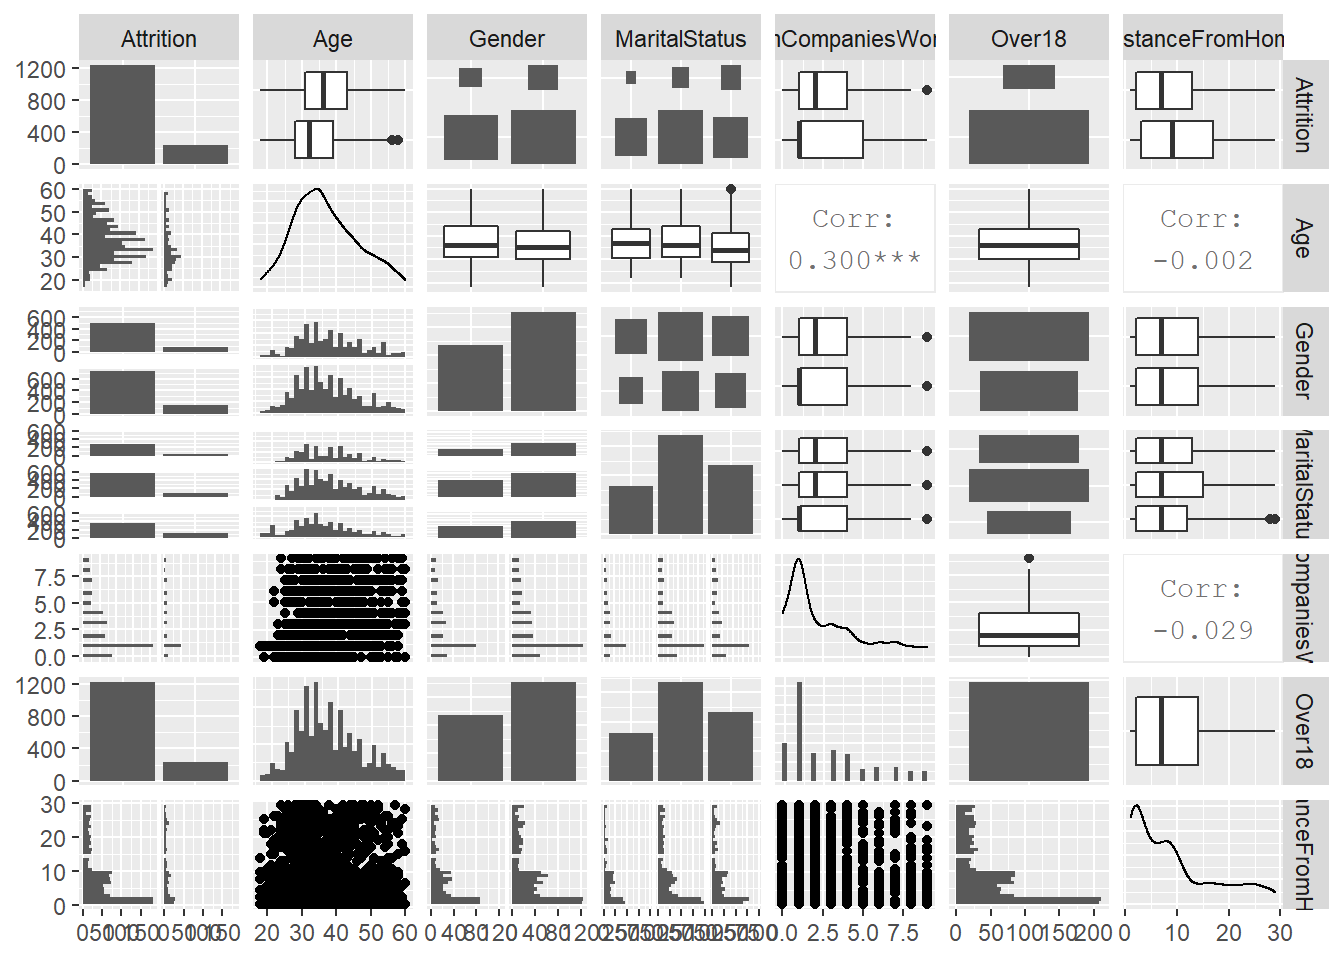
\includegraphics{01_ml_fund_files/figure-latex/unnamed-chunk-2-4.pdf}

\begin{Shaded}
\begin{Highlighting}[]
\NormalTok{employee_attrition_tbl }\OperatorTok
\StringTok{  }\KeywordTok{select}\NormalTok{(Attrition, Age, Gender, MaritalStatus, NumCompaniesWorked, Over18, DistanceFromHome) }\OperatorTok
\StringTok{  }\KeywordTok{ggpairs}\NormalTok{(}\KeywordTok{aes}\NormalTok{(}\DataTypeTok{color =}\NormalTok{ Attrition), }\DataTypeTok{lower =} \StringTok{"blank"}\NormalTok{, }\DataTypeTok{legend =} \DecValTok{1}\NormalTok{,}
          \DataTypeTok{diag  =} \KeywordTok{list}\NormalTok{(}\DataTypeTok{continuous =} \KeywordTok{wrap}\NormalTok{(}\StringTok{"densityDiag"}\NormalTok{, }\DataTypeTok{alpha =} \FloatTok{0.5}\NormalTok{))) }\OperatorTok{+}
\StringTok{  }\KeywordTok{theme}\NormalTok{(}\DataTypeTok{legend.position =} \StringTok{"bottom"}\NormalTok{)}
\end{Highlighting}
\end{Shaded}

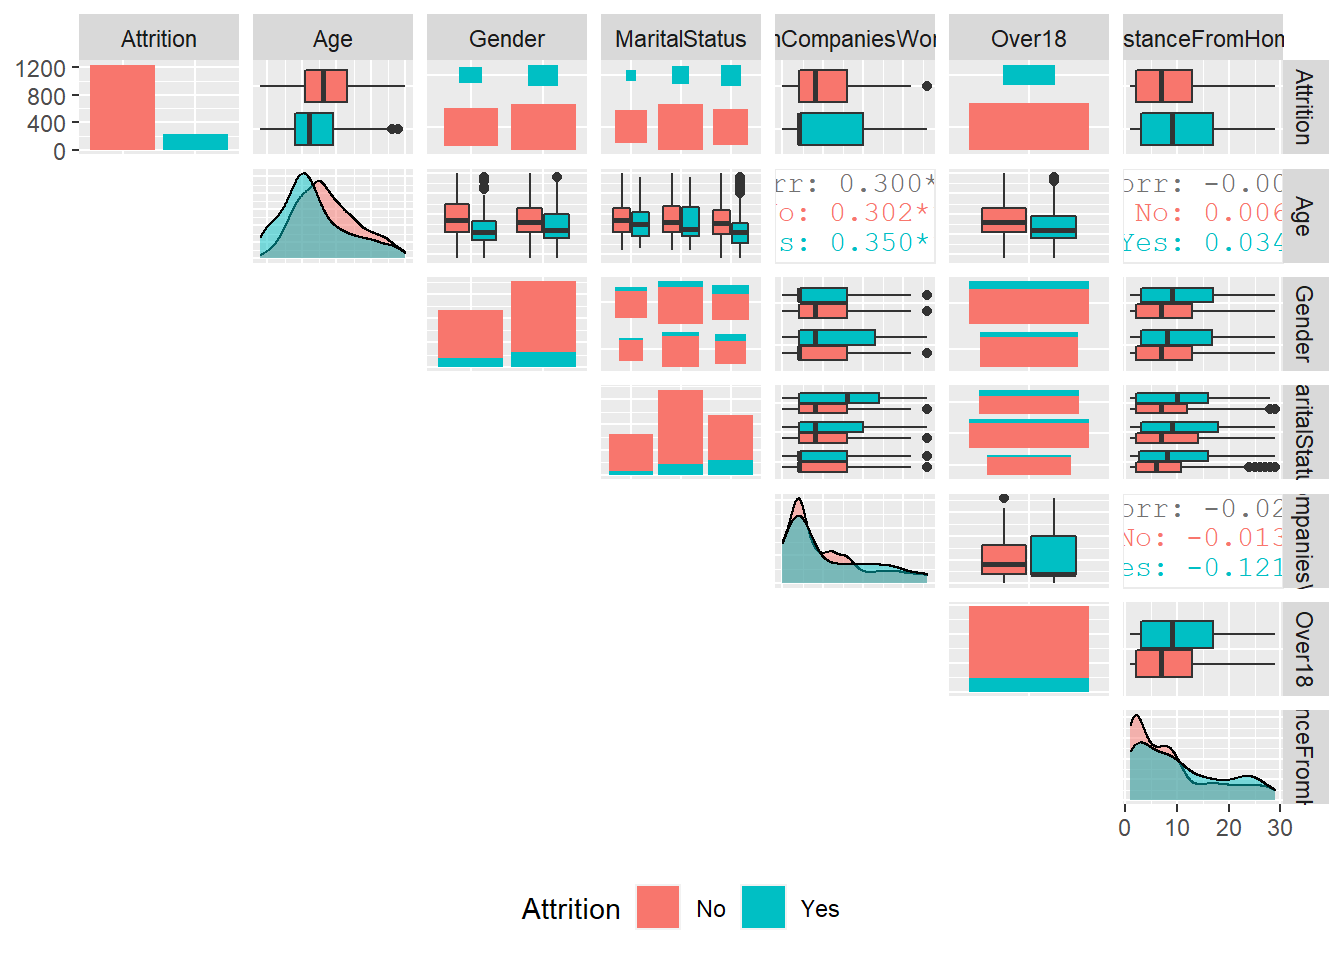
\includegraphics{01_ml_fund_files/figure-latex/unnamed-chunk-2-5.pdf}

\begin{Shaded}
\begin{Highlighting}[]
\CommentTok{# Create data tibble, to potentially debug the plot_ggpairs function (because it has a data argument)}
\NormalTok{data <-}\StringTok{ }\NormalTok{employee_attrition_tbl }\OperatorTok
\StringTok{  }\KeywordTok{select}\NormalTok{(Attrition, Age, Gender, MaritalStatus, NumCompaniesWorked, Over18, DistanceFromHome)}

\NormalTok{plot_ggpairs <-}\StringTok{ }\ControlFlowTok{function}\NormalTok{(data, }\DataTypeTok{color =} \OtherTok{NULL}\NormalTok{, }\DataTypeTok{density_alpha =} \FloatTok{0.5}\NormalTok{) \{}

\NormalTok{  color_expr <-}\StringTok{ }\KeywordTok{enquo}\NormalTok{(color)}

  \ControlFlowTok{if}\NormalTok{ (rlang}\OperatorTok{::}\KeywordTok{quo_is_null}\NormalTok{(color_expr)) \{}

\NormalTok{    g <-}\StringTok{ }\NormalTok{data }\OperatorTok
\StringTok{      }\KeywordTok{ggpairs}\NormalTok{(}\DataTypeTok{lower =} \StringTok{"blank"}\NormalTok{)}

\NormalTok{  \} }\ControlFlowTok{else}\NormalTok{ \{}

\NormalTok{    color_name <-}\StringTok{ }\KeywordTok{quo_name}\NormalTok{(color_expr)}

\NormalTok{    g <-}\StringTok{ }\NormalTok{data }\OperatorTok
\StringTok{      }\KeywordTok{ggpairs}\NormalTok{(}\DataTypeTok{mapping =} \KeywordTok{aes_string}\NormalTok{(}\DataTypeTok{color =}\NormalTok{ color_name),}
              \DataTypeTok{lower =} \StringTok{"blank"}\NormalTok{, }\DataTypeTok{legend =} \DecValTok{1}\NormalTok{,}
              \DataTypeTok{diag =} \KeywordTok{list}\NormalTok{(}\DataTypeTok{continuous =} \KeywordTok{wrap}\NormalTok{(}\StringTok{"densityDiag"}\NormalTok{,}
                                            \DataTypeTok{alpha =}\NormalTok{ density_alpha))) }\OperatorTok{+}
\StringTok{      }\KeywordTok{theme}\NormalTok{(}\DataTypeTok{legend.position =} \StringTok{"bottom"}\NormalTok{)}
\NormalTok{  \}}

  \KeywordTok{return}\NormalTok{(g)}

\NormalTok{\}}
\end{Highlighting}
\end{Shaded}

\hypertarget{q1}{%
\subsection{Q1:}\label{q1}}

The answer is C

\begin{Shaded}
\begin{Highlighting}[]
\CommentTok{#Q1}
\NormalTok{employee_attrition_tbl }\OperatorTok
\StringTok{  }\KeywordTok{select}\NormalTok{(Attrition, }\KeywordTok{contains}\NormalTok{(}\StringTok{"income"}\NormalTok{)) }\OperatorTok
\StringTok{  }\KeywordTok{plot_ggpairs}\NormalTok{(Attrition)}
\end{Highlighting}
\end{Shaded}

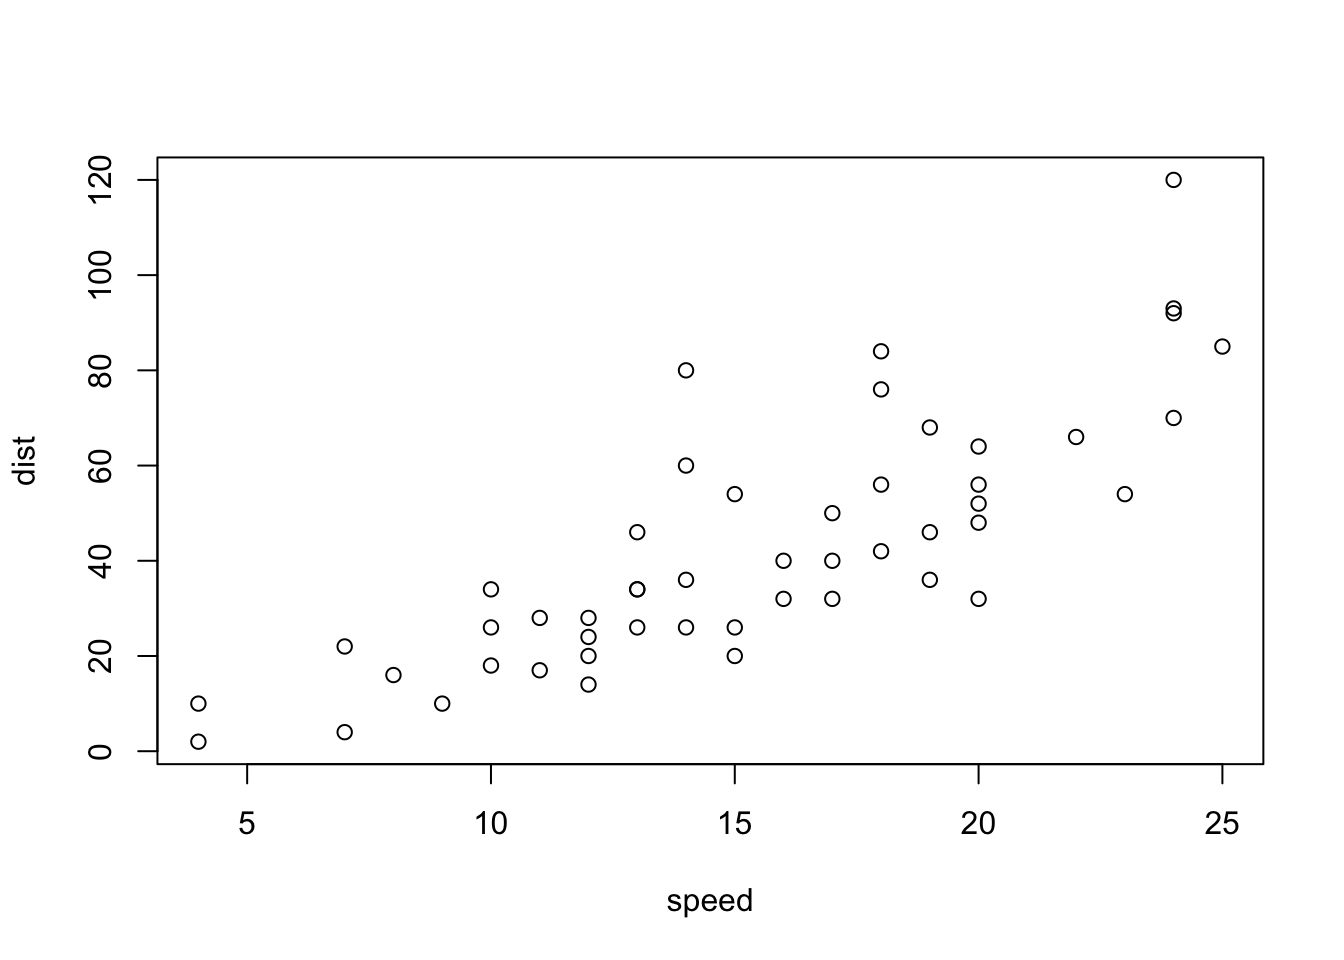
\includegraphics{01_ml_fund_files/figure-latex/unnamed-chunk-3-1.pdf}

\begin{Shaded}
\begin{Highlighting}[]
\CommentTok{#The answer is C}
\end{Highlighting}
\end{Shaded}

\hypertarget{q2}{%
\subsection{Q2:}\label{q2}}

The answer is D

\begin{Shaded}
\begin{Highlighting}[]
\CommentTok{#Q2}
\NormalTok{employee_attrition_tbl }\OperatorTok
\StringTok{  }\KeywordTok{select}\NormalTok{(Attrition, }\KeywordTok{contains}\NormalTok{(}\StringTok{"PercentSalaryHike"}\NormalTok{)) }\OperatorTok
\StringTok{  }\KeywordTok{plot_ggpairs}\NormalTok{(Attrition)}
\end{Highlighting}
\end{Shaded}

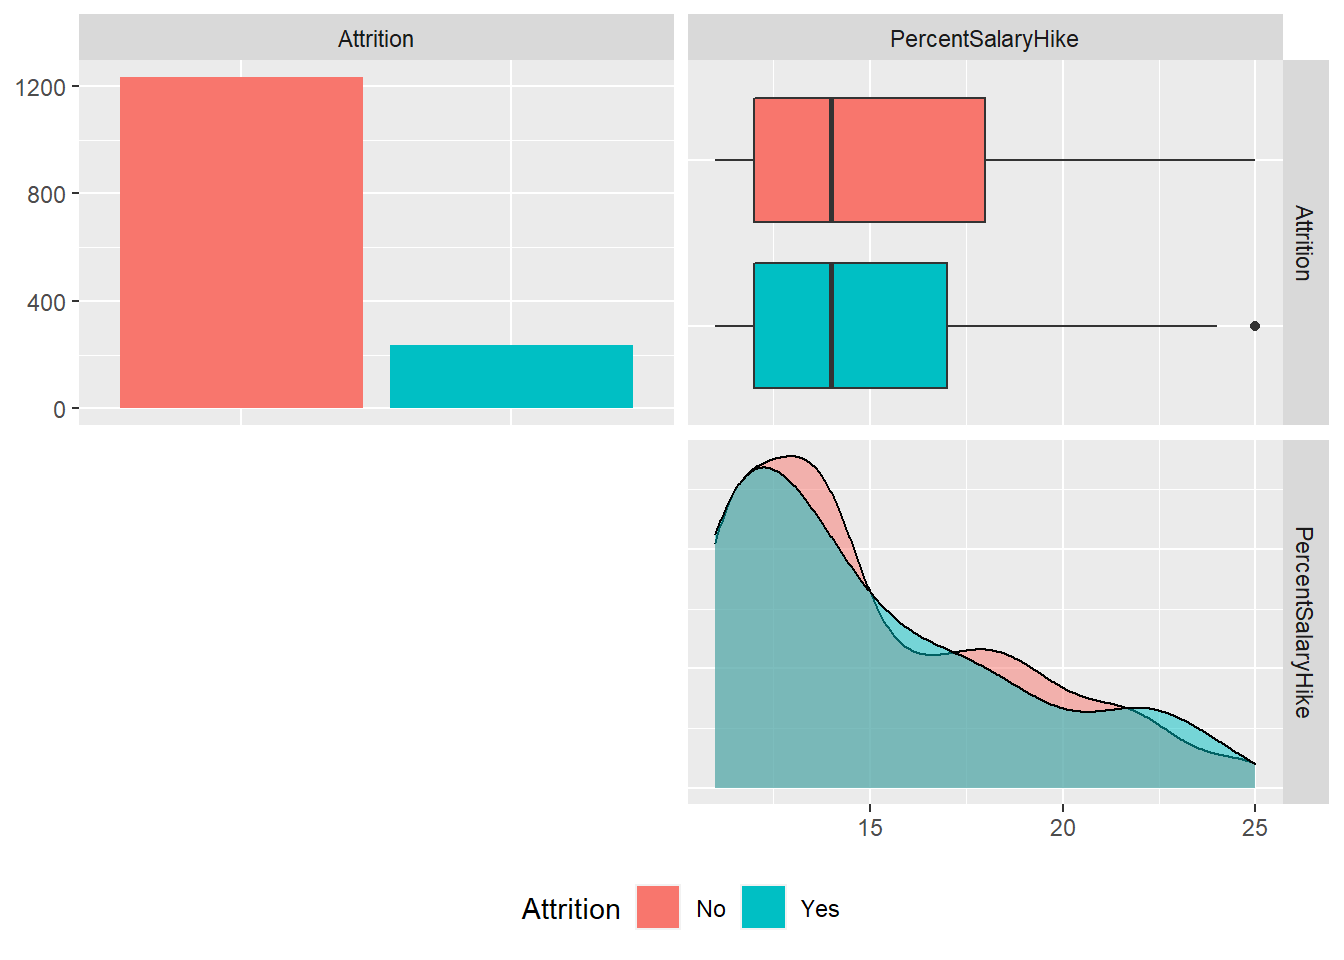
\includegraphics{01_ml_fund_files/figure-latex/unnamed-chunk-4-1.pdf}

\begin{Shaded}
\begin{Highlighting}[]
\CommentTok{#The answer is D}
\end{Highlighting}
\end{Shaded}

\hypertarget{q3}{%
\subsection{Q3}\label{q3}}

The answer is B

\begin{Shaded}
\begin{Highlighting}[]
\CommentTok{#Q3}
\NormalTok{employee_attrition_tbl }\OperatorTok
\StringTok{  }\KeywordTok{select}\NormalTok{(Attrition, }\KeywordTok{contains}\NormalTok{(}\StringTok{"StockOptionLevel"}\NormalTok{)) }\OperatorTok
\StringTok{  }\KeywordTok{plot_ggpairs}\NormalTok{(Attrition)}
\end{Highlighting}
\end{Shaded}

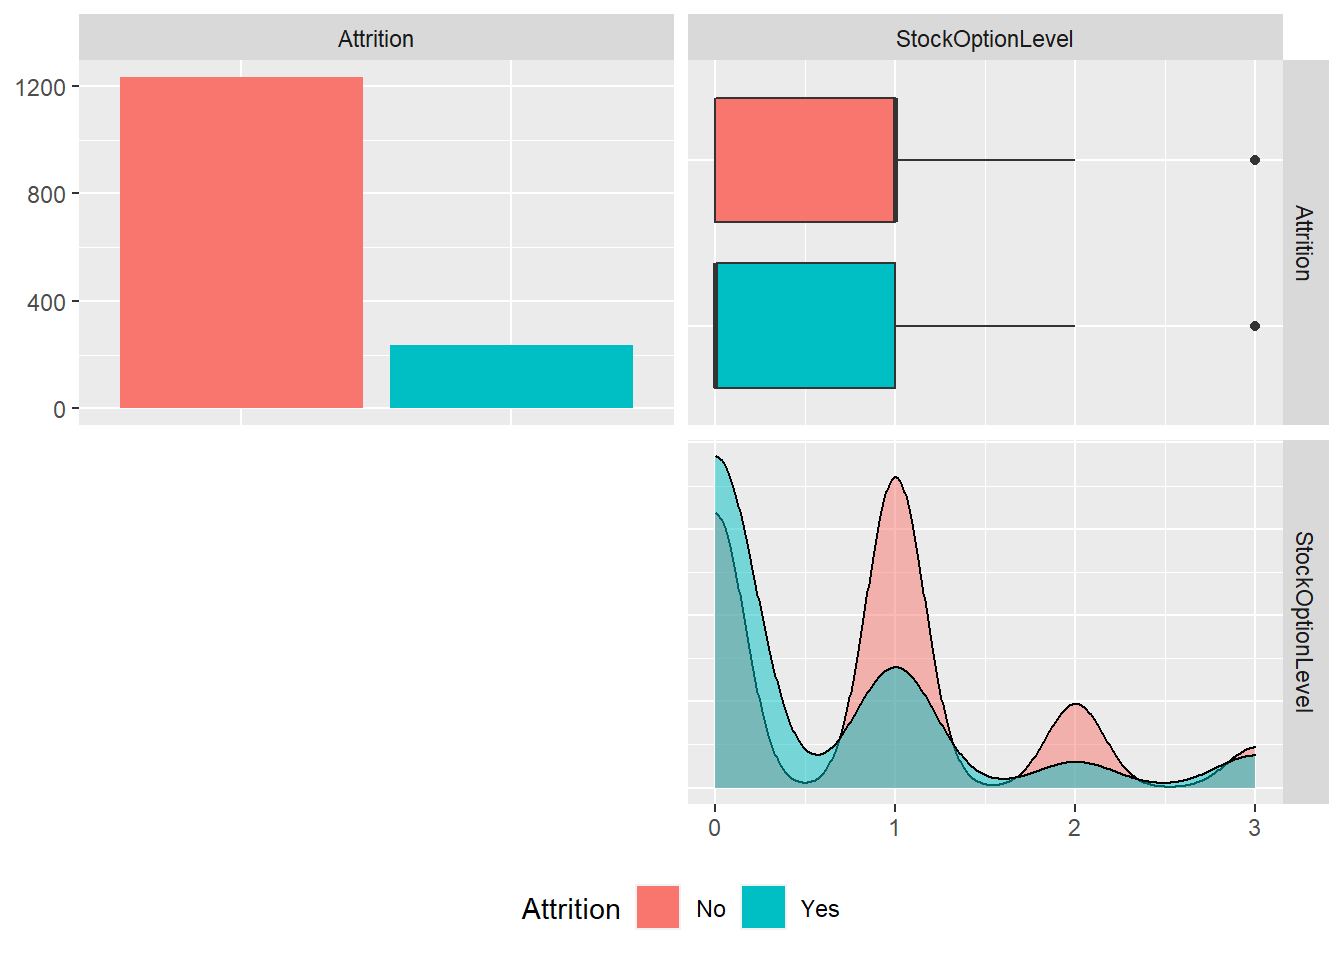
\includegraphics{01_ml_fund_files/figure-latex/unnamed-chunk-5-1.pdf}

\begin{Shaded}
\begin{Highlighting}[]
\CommentTok{#The answer is B}
\end{Highlighting}
\end{Shaded}

\hypertarget{q4}{%
\subsection{Q4}\label{q4}}

The answer is A

\begin{Shaded}
\begin{Highlighting}[]
\CommentTok{#Q4}

\NormalTok{employee_attrition_tbl }\OperatorTok
\StringTok{  }\KeywordTok{select}\NormalTok{(Attrition, }\KeywordTok{contains}\NormalTok{(}\StringTok{"EnvironmentSatisfaction"}\NormalTok{)) }\OperatorTok
\StringTok{  }\KeywordTok{plot_ggpairs}\NormalTok{(Attrition)}
\end{Highlighting}
\end{Shaded}

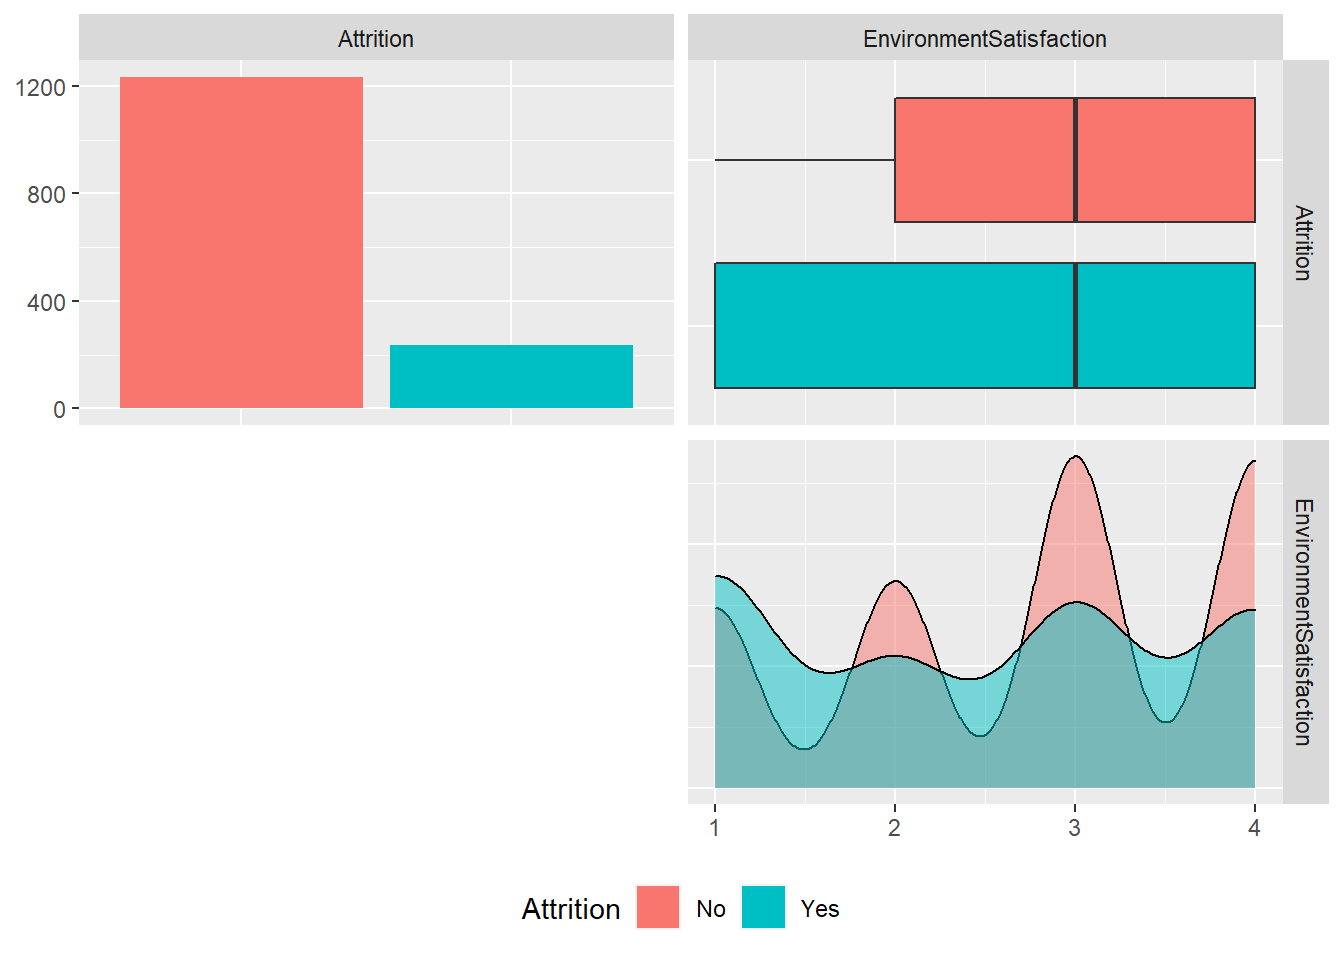
\includegraphics{01_ml_fund_files/figure-latex/unnamed-chunk-6-1.pdf}

\begin{Shaded}
\begin{Highlighting}[]
\CommentTok{#The answer is A}
\end{Highlighting}
\end{Shaded}

\hypertarget{q5}{%
\subsection{Q5}\label{q5}}

The answer is B

\begin{Shaded}
\begin{Highlighting}[]
\CommentTok{#Q5}

\NormalTok{employee_attrition_tbl }\OperatorTok
\StringTok{  }\KeywordTok{select}\NormalTok{(Attrition, }\KeywordTok{contains}\NormalTok{(}\StringTok{"WorkLifeBalance"}\NormalTok{)) }\OperatorTok
\StringTok{  }\KeywordTok{plot_ggpairs}\NormalTok{(Attrition)}
\end{Highlighting}
\end{Shaded}

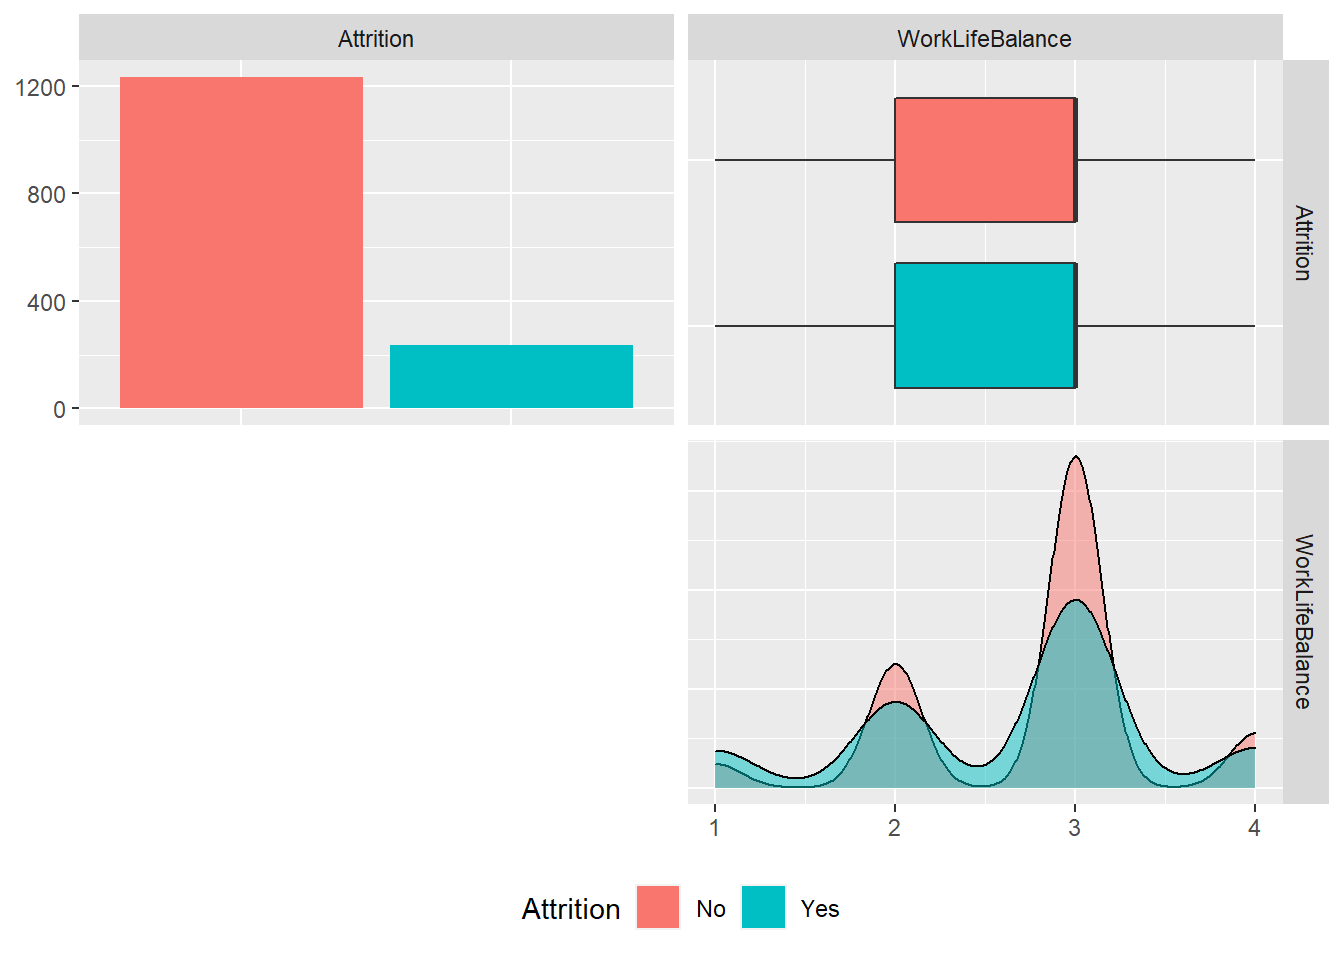
\includegraphics{01_ml_fund_files/figure-latex/unnamed-chunk-7-1.pdf}

\begin{Shaded}
\begin{Highlighting}[]
\CommentTok{#The answer is B}
\end{Highlighting}
\end{Shaded}

\hypertarget{q6}{%
\subsection{Q6}\label{q6}}

The answer is A

\begin{Shaded}
\begin{Highlighting}[]
\CommentTok{#Q6}

\NormalTok{employee_attrition_tbl }\OperatorTok
\StringTok{  }\KeywordTok{select}\NormalTok{(Attrition, }\KeywordTok{contains}\NormalTok{(}\StringTok{"JobInvolvement"}\NormalTok{)) }\OperatorTok
\StringTok{  }\KeywordTok{plot_ggpairs}\NormalTok{(Attrition)}
\end{Highlighting}
\end{Shaded}

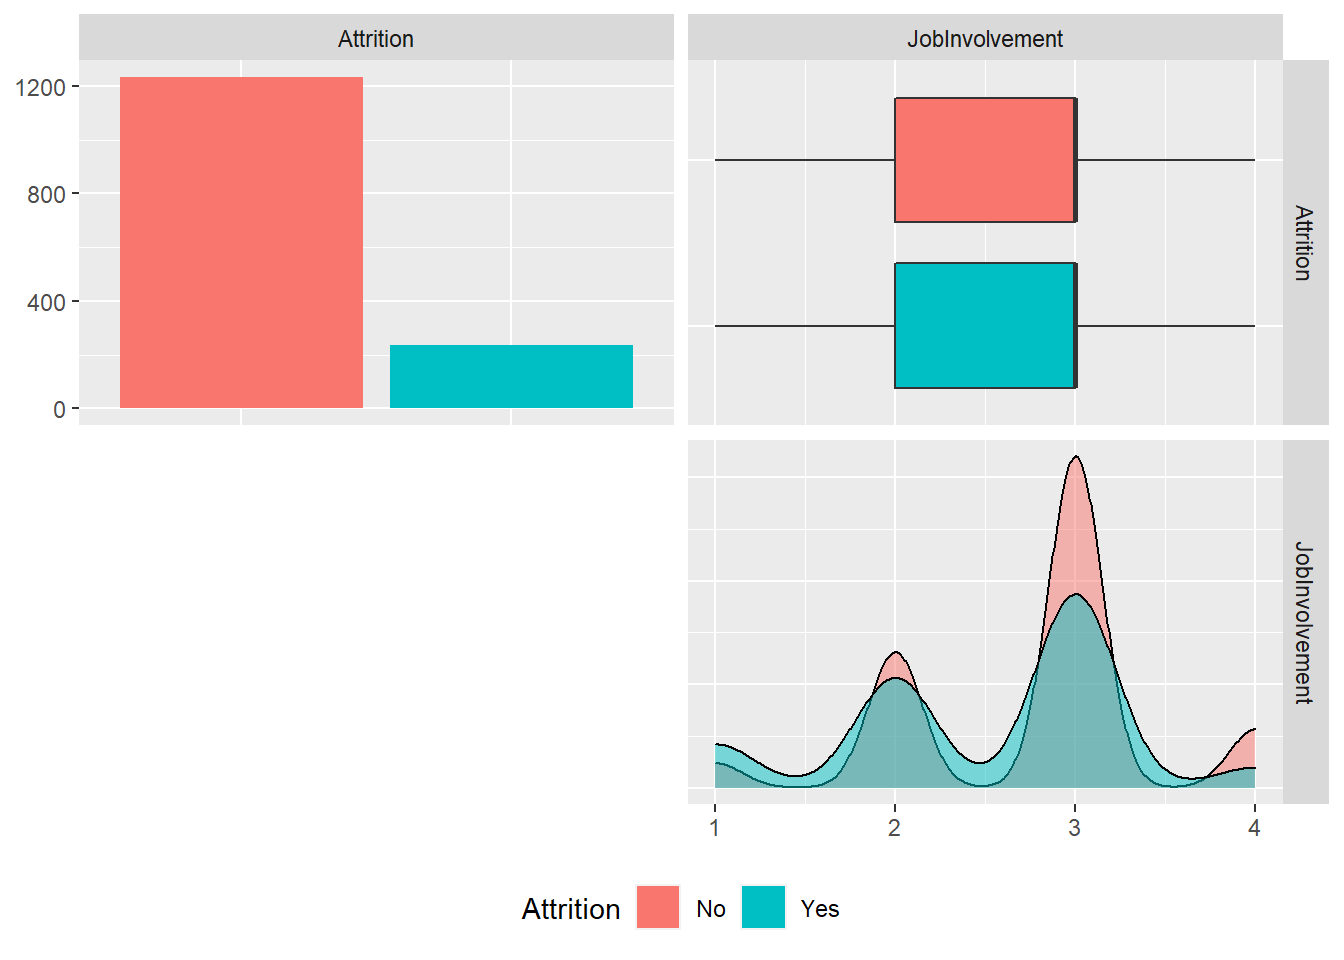
\includegraphics{01_ml_fund_files/figure-latex/unnamed-chunk-8-1.pdf}

\begin{Shaded}
\begin{Highlighting}[]
\CommentTok{#The answer is A}
\end{Highlighting}
\end{Shaded}

\hypertarget{q7}{%
\subsection{Q7}\label{q7}}

The answer is B

\begin{Shaded}
\begin{Highlighting}[]
\CommentTok{#Q7}
\NormalTok{employee_attrition_tbl }\OperatorTok
\StringTok{  }\KeywordTok{select}\NormalTok{(Attrition, }\KeywordTok{contains}\NormalTok{(}\StringTok{"OverTime"}\NormalTok{)) }\OperatorTok
\StringTok{  }\KeywordTok{plot_ggpairs}\NormalTok{(Attrition)}
\end{Highlighting}
\end{Shaded}

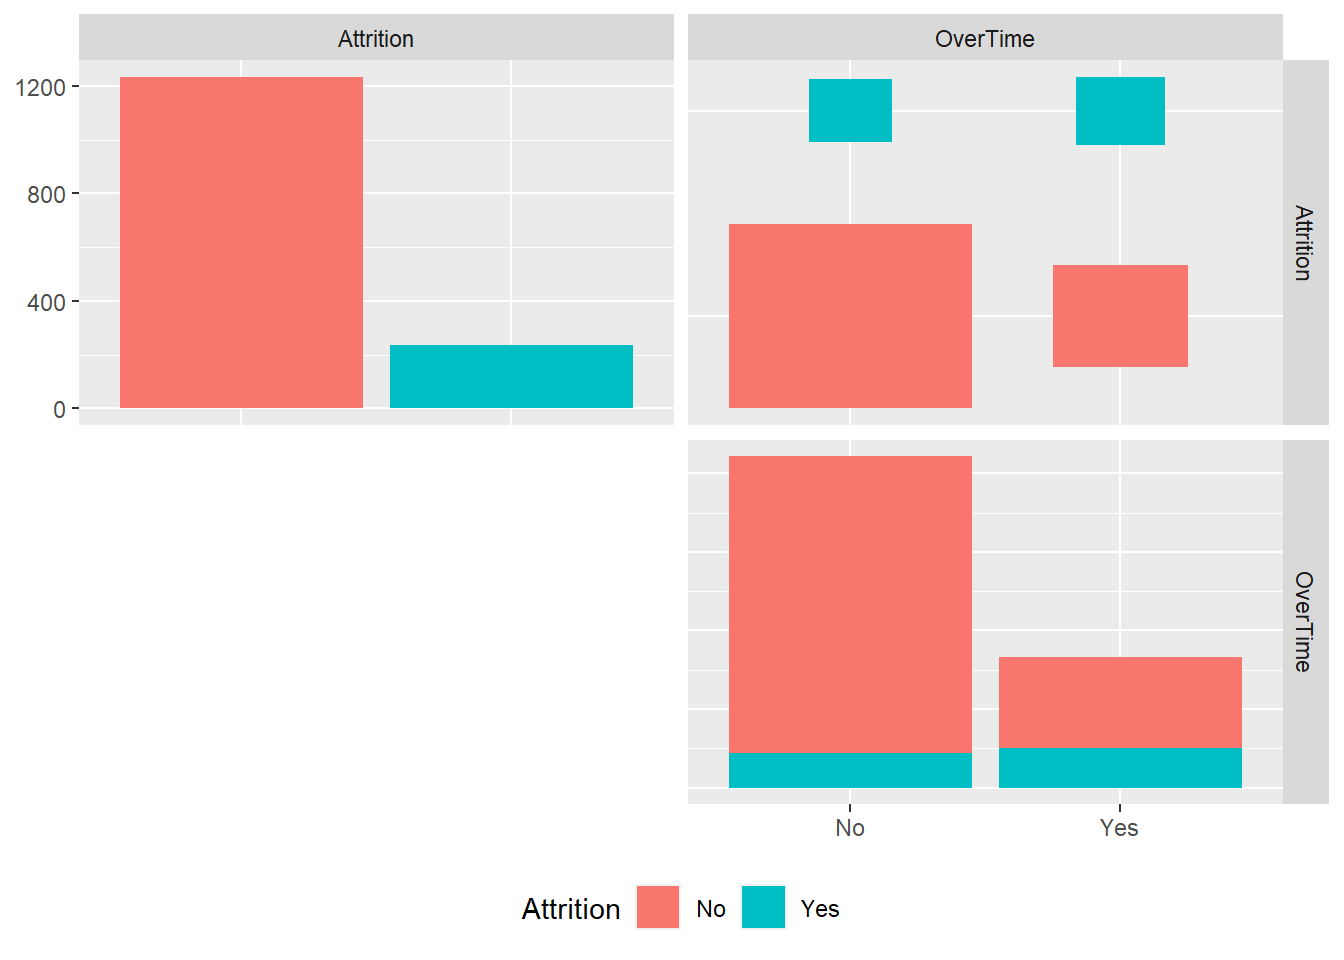
\includegraphics{01_ml_fund_files/figure-latex/unnamed-chunk-9-1.pdf}

\begin{Shaded}
\begin{Highlighting}[]
\CommentTok{#The answer is B}
\end{Highlighting}
\end{Shaded}

\hypertarget{q8}{%
\subsection{Q8}\label{q8}}

The answer is B

\begin{Shaded}
\begin{Highlighting}[]
\CommentTok{#Q8}
\NormalTok{employee_attrition_tbl }\OperatorTok
\StringTok{  }\KeywordTok{select}\NormalTok{(Attrition, }\KeywordTok{contains}\NormalTok{(}\StringTok{"TrainingTimesLastYear"}\NormalTok{)) }\OperatorTok
\StringTok{  }\KeywordTok{plot_ggpairs}\NormalTok{(Attrition)}
\end{Highlighting}
\end{Shaded}

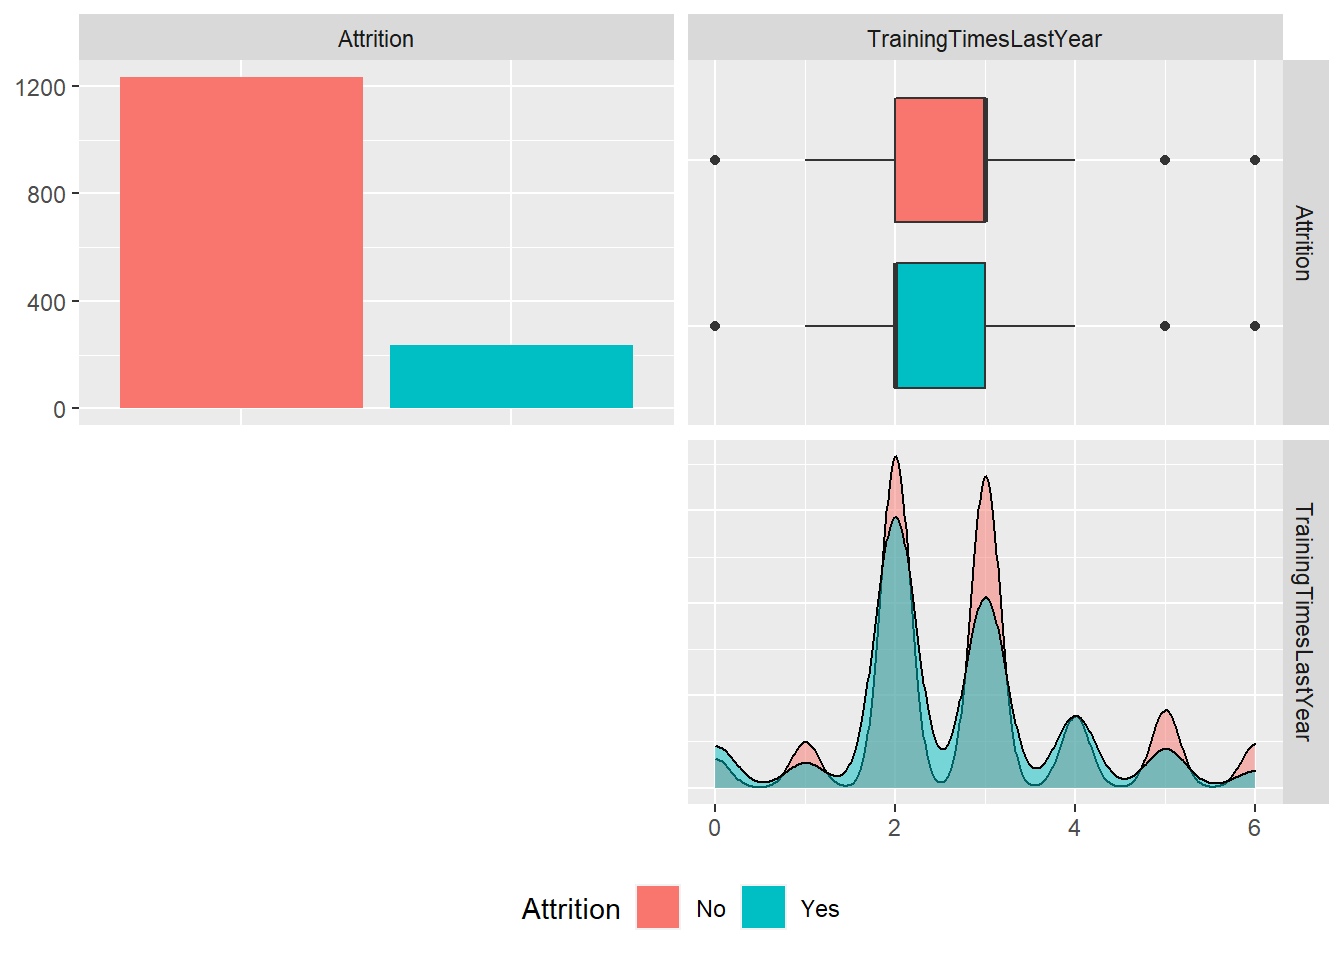
\includegraphics{01_ml_fund_files/figure-latex/unnamed-chunk-10-1.pdf}

\begin{Shaded}
\begin{Highlighting}[]
\CommentTok{#The answer is B}
\end{Highlighting}
\end{Shaded}

\hypertarget{q9}{%
\subsection{Q9}\label{q9}}

The answer is B

\begin{Shaded}
\begin{Highlighting}[]
\CommentTok{#Q9}
\NormalTok{employee_attrition_tbl }\OperatorTok
\StringTok{  }\KeywordTok{select}\NormalTok{(Attrition, }\KeywordTok{contains}\NormalTok{(}\StringTok{"YearsAtCompany"}\NormalTok{)) }\OperatorTok
\StringTok{  }\KeywordTok{plot_ggpairs}\NormalTok{(Attrition)}
\end{Highlighting}
\end{Shaded}

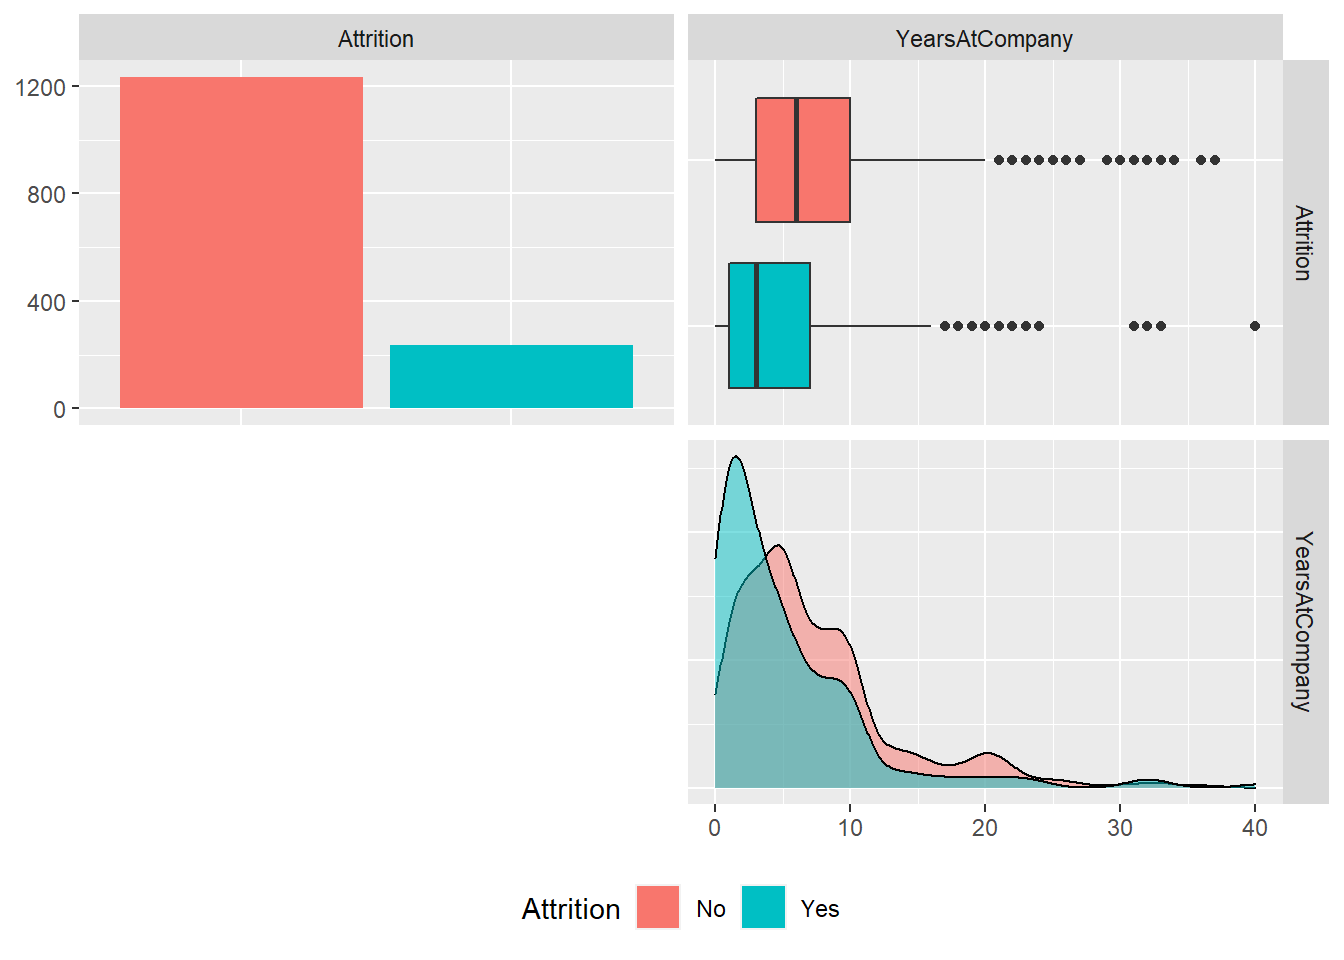
\includegraphics{01_ml_fund_files/figure-latex/unnamed-chunk-11-1.pdf}

\begin{Shaded}
\begin{Highlighting}[]
\CommentTok{#The answer is B}
\end{Highlighting}
\end{Shaded}

\hypertarget{q10}{%
\subsection{Q10}\label{q10}}

The answer is C

\begin{Shaded}
\begin{Highlighting}[]
\CommentTok{#Q 10}
\NormalTok{employee_attrition_tbl }\OperatorTok
\StringTok{  }\KeywordTok{select}\NormalTok{(Attrition, }\KeywordTok{contains}\NormalTok{(}\StringTok{"YearsSinceLastPromotion"}\NormalTok{)) }\OperatorTok
\StringTok{  }\KeywordTok{plot_ggpairs}\NormalTok{(Attrition)}
\end{Highlighting}
\end{Shaded}

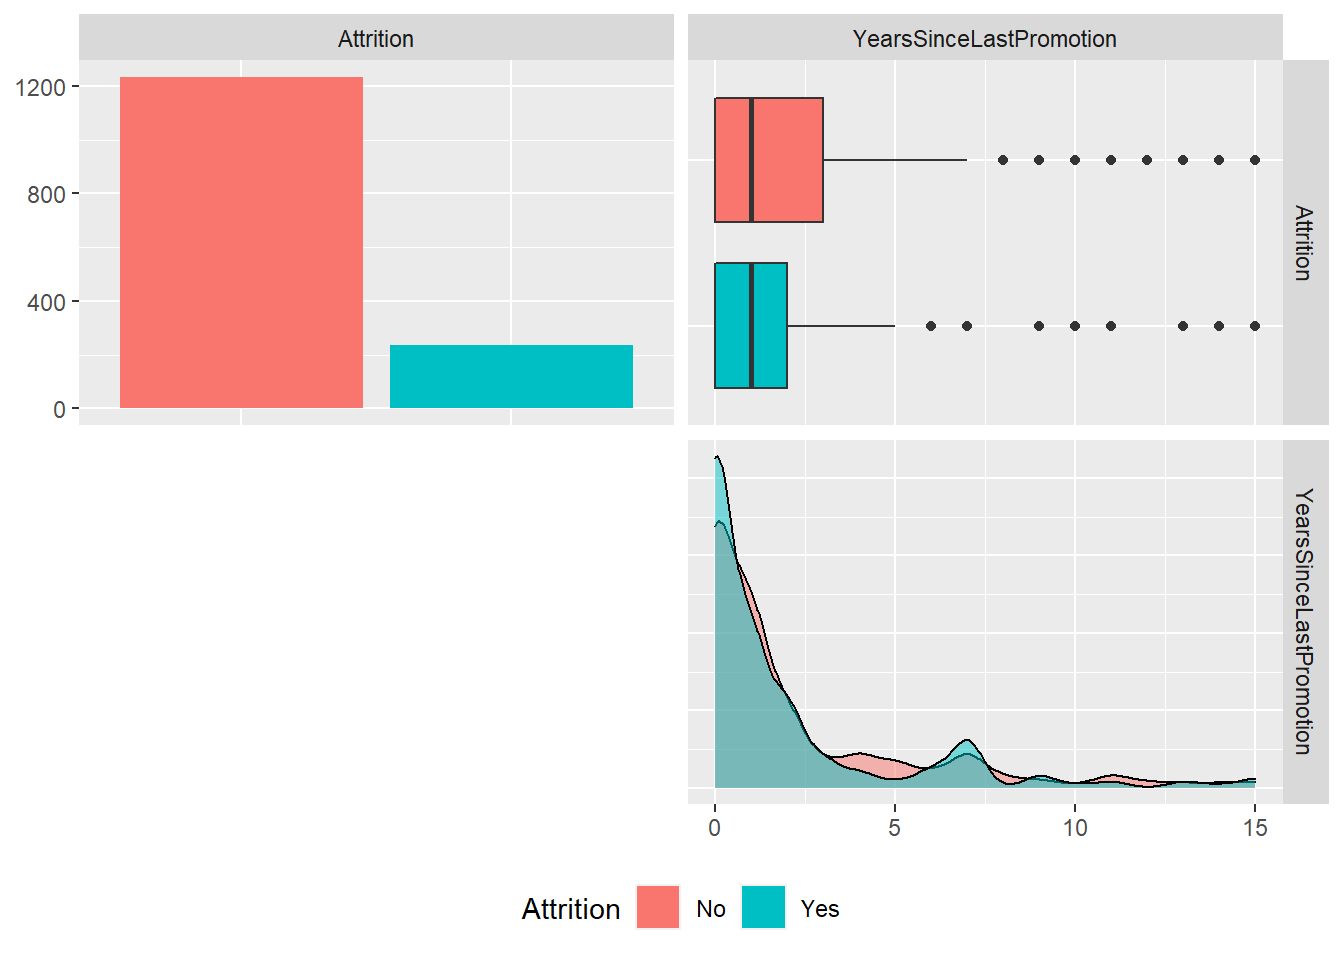
\includegraphics{01_ml_fund_files/figure-latex/unnamed-chunk-12-1.pdf}

\begin{Shaded}
\begin{Highlighting}[]
\CommentTok{#The answer is C}
\end{Highlighting}
\end{Shaded}

\end{document}
